% Contenidos del capítulo.
% Las secciones presentadas son orientativas y no representan
% necesariamente la organización que debe tener este capítulo.
Este capítulo tiene como objetivo detallar la implementación técnica de los distintos subsistemas que conforman el sistema, conforme a la arquitectura previamente definida. En primer lugar, se abordará la codificación e integración de los componentes pertenecientes a cada nodo funcional, siguiendo el orden lógico de ejecución dentro del flujo del sistema. A continuación, se describirá el funcionamiento global del sistema, incluyendo su proceso de despliegue local para la gestión de los servicios. Finalmente, se presentará el diseño y ejecución de un conjunto de pruebas funcionales y de rendimiento, orientadas a validar la estabilidad y eficiencia del sistema implementado.


\section{Implementación del subsistema del add-on de Blender}
En primer lugar, nos enfocaremos en la implementación del subsistema inicial, el cual corresponde al complemento específico de Blender que establecerá la conexión, a través de la interfaz gráfica, entre el usuario/a y los distintos servicios ofrecidos por el servidor de inteligencias artificiales. Además de facilitar esta conexión, el complemento desempeña otras funciones como la ejecución del código generado en la respuesta, la importación de imágenes, la exportación de modelos 3D, la carga de modelos 3D en la escena de Blender, la reversión de cualquier modificación realizada en la escena mediante el complemento y la visualización de cualquier error que ocurra durante su uso. Cabe destacar que la implementación de este subsistema se ha estructurado en tres etapas primeramente, la implementación de la interfaz gráfica y su correspondiente infraestructura secundaria, en segundo lugar, la implementación de la llamada para la generación del modelo 3D y finalmente, la llamada para la generación de texto del modelo \gls{llm}.
La Figura \ref{fig:instAddonBlender} muestra el panel de preferencias de Blender correspondiente a la versión 3.6 LTS, desde el cual se gestiona la instalación de complementos (add-ons). Para que el proceso de carga sea exitoso, es necesario empaquetar el conjunto de archivos del complemento en un archivo comprimido con extensión \verb|.zip|. Asimismo, se requiere que el archivo principal del complemento esté correctamente nombrado como \verb|__init__.py|, en conformidad con la estructura exigida por el sistema de detección e integración automática de Blender. Esta convención ha sido seguida en la implementación del presente trabajo.

% Imagen instalación add-on
\begin{figure}[h!tb]
  \centering
  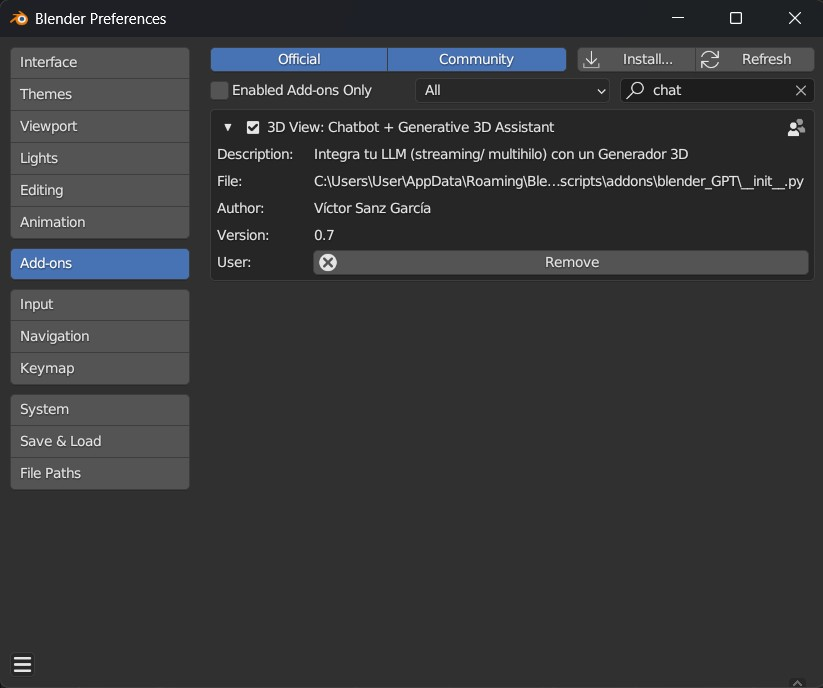
\includegraphics[width=0.8\textwidth]{figs/instalAddon.jpg}
  \caption{Instalación del add-on de Blender.}
  \label{fig:instAddonBlender}
\end{figure}

\subsection{Implementación de la interfaz de usuario y las herramientas auxiliares}
Para el desarrollo de la interfaz de usuario del complemento, se ha utilizado el lenguaje Python, aprovechando la API nativa de Blender, que permite la creación de add-ons personalizados mediante clases y métodos definidos en el módulo \verb|bpy|. En el Listado \ref{lst:panelAddon1} se presenta el código fuente completo de la interfaz, estructurado en un panel incorporado en la barra lateral de la vista 3D. Este panel se implementa mediante una subclase de \verb|bpy.types.Panel|, registrada con los atributos \verb|bl_space_type='VIEW_3D'| y \verb|bl_region_type='UI'|, lo que permite exponer controles gráficos vinculados a propiedades definidas en \verb|bpy.types.Scene|.

La interfaz se divide funcionalmente en dos secciones principales. La primera corresponde al Agente \gls{llm}, que incluye:
\begin{itemize}
  \item Un campo de texto para introducir el prompt del usuario/a.
  \item Un botón asociado que envía el prompt al modelo \gls{llm} para la generación de código.
  \item Un campo de texto para mostrar la respuesta generada por el modelo.
  \item Un botón adicional que ejecuta directamente el código recibido dentro del entorno de Blender.

        Además, una vez se recibe la respuesta, se activa automáticamente el panel de scripting de Blender, donde también se muestra el código generado.
\end{itemize}
La segunda sección está destinada al Agente 3D y contempla el flujo de generación de modelos tridimensionales a partir de imágenes. Esta parte incluye:
\begin{itemize}
  \item Un botón que abre el explorador de archivos para seleccionar la imagen de entrada.
  \item Un botón para enviar la imagen al modelo generativo 3D y recibir la reconstrucción.
  \item Una vez obtenida la respuesta, se habilitan dos botones adicionales, uno para importar el modelo 3D directamente en la escena de Blender y otro para exportarlo en formato \verb|.glb|, permitiendo al usuario/a elegir la ruta de descarga a través del sistema de archivos.
\end{itemize}
El panel del add-on se puede observar en la Figura \ref{fig:addonBlender}.

% Imagen add-on
\begin{figure}[h!tb]
  \centering
  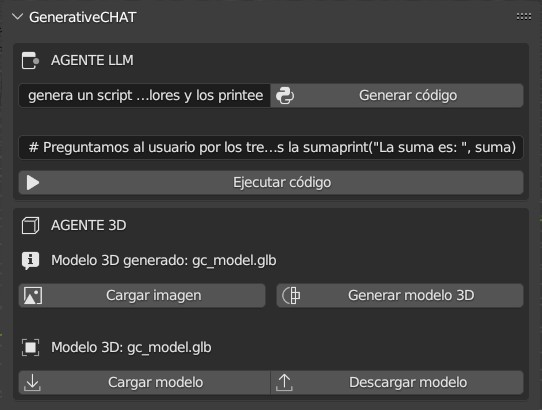
\includegraphics[width=0.8\textwidth]{figs/panelAddon.jpg}
  \caption{Interfaz de usuario del add-on de Blender.}
  \label{fig:addonBlender}
\end{figure}

Para la ejecución dinámica de código Python generado, se ha desarrollado un operador personalizado en Blender que accede al bloque de texto almacenado como propiedad en la escena. La ejecución se realiza mediante la función \verb|exec()| dentro del método \verb|execute(self, context)|, encapsulando el proceso en una estructura de control \verb|try/except| que permite capturar y reportar posibles errores mediante \verb|self.report|, sin comprometer la estabilidad ni bloquear la interfaz de usuario. La importación de imágenes se gestiona a través de otro operador que utiliza el selector de archivos \\(\verb|context.window_manager|), y una vez seleccionada la imagen, se carga en memoria con \verb|bpy.data.images.load()|. La ruta y el nombre del datablock correspondiente se almacenan en propiedades de escena para su reutilización, y se presenta una vista previa mediante \verb|layout.template_preview(img)| para validar visualmente la carga. En cuanto a la exportación de modelos 3D, se implementa un operador que invoca un diálogo de guardado, y dentro del método \verb|execute()| transfiere el archivo temporal (en formato \verb|.glb|) a la ruta de destino utilizando \verb|shutil.copy|. Este proceso también contempla el manejo de excepciones relacionadas con permisos o rutas inexistentes, notificando al usuario/a mediante los correspondientes mensajes de error. Para la carga de modelos 3D en la escena, se ha definido otro operador que verifica la validez de la ruta previamente almacenada y realiza la importación a través de \verb|bpy.ops.import_scene.gltf(filepath=...)| adecuado para el formato \verb|.glb|. Se implementan bloques \verb|try/except| tanto para informar errores como para confirmar el éxito del proceso. Las funcionalidades de reversión de cambios aprovechan el sistema de deshacer nativo de Blender, mediante la declaración \verb|bl_options = {'REGISTER', 'UNDO'}| en aquellos operadores que modifican el estado de la escena. Esto permite que cualquier acción pueda ser revertida mediante combinaciones estándar como Ctrl+Z. Durante todo el flujo, se emplea una propiedad de estado en la escena para mostrar mensajes persistentes de seguimiento por ejemplo, (Generando...) y (Error...), actualizados desde el hilo principal mediante \verb|bpy.app.timers.register| en casos donde se recurre a procesos asincrónicos como llamadas HTTP. Esto asegura que la interfaz de usuario permanezca reactiva, incluso durante operaciones de larga duración. Finalmente, todos los operadores implementan validaciones previas sobre las rutas y datos implicados, gestionan adecuadamente los nombres de los datablocks para evitar colisiones y realizan limpieza de recursos temporales cuando es necesario. Se han incluido además descripciones (\verb|bl_description|) y docstrings claras en cada clase, mejorando la usabilidad, la documentación interna y la detección de errores por parte del usuario/a durante la ejecución de tareas críticas como importación, exportación o ejecución de scripts generados dinámicamente.




\subsection{Implementación de la llamada al modelo 3D}
Para implementar la funcionalidad de llamada al modelo generativo 3D en el add-on de Blender, se ha diseñado un operador personalizado (ver Listado \ref{lst:panelAddon1}) que emplea un hilo secundario (thread) para realizar la solicitud HTTP al servicio de generación de modelos 3D desplegado en el puerto 5000 del localhost (\verb|http://127.0.0.1:5000/upload|) que se explica posteriormente en la implementación del subsistema del servidor, con el objetivo de mantener la interfaz de usuario no bloqueante durante el proceso. En el método \verb|execute()|, se lanza un \verb|threading.Thread| en modo daemon, encargado de ejecutar la función \verb|requests.post| con la imagen seleccionada como entrada. Dado que la API de Blender no es segura para operaciones multihilo, no se realiza ninguna modificación directa sobre \verb|bpy.data| ni \verb|bpy.context| desde este hilo. En su lugar, se emplea una estructura de cola (\verb|queue.Queue|) para transferir el resultado de la petición al hilo principal. La comunicación asincrónica se gestiona mediante el registro de una función de callback en \verb|bpy.app.timers.register|, la cual se ejecuta en el hilo principal cuando la respuesta esté disponible. Este callback evalúa si la respuesta HTTP ha sido satisfactoria: si es así, guarda el archivo \verb|.glb| generado en una ruta temporal (usando \verb|tempfile.gettempdir()|), actualiza la propiedad\\ \verb|scene.gc_model_path| y modifica el estado \verb|scene.gc_status| con un mensaje del tipo “Modelo generado: nombre.glb”. En caso de producirse errores durante la solicitud (por ejemplo, fallos de red, timeouts o respuestas mal formateadas), estos se capturan en el hilo secundario y se comunican al principal mediante la cola. El callback en el hilo principal ejecuta un bloque \verb|try/except| para gestionar estos errores, actualizando el estado de la escena (\verb|scene.gc_status = f"Error: {str(e)}"|) y notificando al usuario/a mediante \verb|self.report({'ERROR'}, ...)|, ya sea dentro del operador inicial o mediante un operador auxiliar de notificación. Esta arquitectura garantiza que todas las interacciones con la API de Blender se realicen exclusivamente en el hilo principal, respetando las restricciones de seguridad asociadas a su ejecución. Durante todo el proceso, el panel de interfaz de usuario refleja el estado del sistema mostrando el mensaje “Generando…” mientras la operación está en curso. Una vez el callback actualiza el estado, se habilitan dinámicamente los botones “Cargar modelo” y “Descargar modelo”, o en su defecto, se muestra un mensaje de error.



\subsection{Implementación de la llamada al modelo LLM}

El Listado \ref{lst:streamBotAddon} detalla la implementación de la petición al modelo de lenguaje LLM.
Esta implementación se basa en una función denominada \verb|chatbot(pmt, key)|, la cual construye y envía una solicitud HTTP de tipo POST con soporte para transmisión continua de datos (streaming) al punto de acceso local (\verb|http://127.0.0.1:11434/api/generate|) expuesto en el puerto 11434 del localhost, lo cual se detalla posteriormente en la implementación de la arquitectura del subsistema del servidor. El cuerpo de la solicitud contiene un objeto JSON que incluye tanto el mensaje del usuario/a como los parámetros de configuración del modelo, tales como la selección del modelo específico \\(\verb|"model": "dolphin-mistral:7b-v2.6-dpo-laser-q4_0"|) y la activación del modo de respuesta continua (\verb|"stream": true|). La respuesta del servidor se gestiona de forma iterativa utilizando \verb|response.iter_lines()|, lo que permite procesar fragmentos de texto en tiempo real conforme son recibidos, evitando así bloqueos durante la generación de contenido. Cada línea de la respuesta es tratada como una posible estructura JSON. Si se detecta la presencia del campo \verb|response|, el fragmento correspondiente se extrae y se transmite a una cola de procesamiento (\verb|queue.Queue|) mediante la instrucción \verb|q.put(chunk)|. Este flujo se encapsula en una función \verb|create_chat_bot|, que actúa como envoltorio para ejecutar \verb|chatbot| dentro de un hilo secundario. Esta estrategia multihilo permite invocar la función desde el operador de Blender sin interferir con el hilo principal de la interfaz gráfica.
En el hilo principal, se utiliza \verb|bpy.app.timers.register(process_queue)| para programar un temporizador que accede periódicamente a la cola, extrayendo los fragmentos generados y pasándolos a la función \verb|write_chat(chunk)|. Esta función acumula el contenido en una variable global, filtra mediante expresiones regulares los bloques de código Python delimitados, y los inserta en un datablock de texto dentro de Blender. Simultáneamente, se actualiza la propiedad \verb|scene.response| para reflejar el resultado filtrado en la interfaz de usuario. El manejo de errores en la interacción con el modelo \gls{llm} se gestiona mediante bloques \verb|try/except| en la función \verb|chatbot|, donde se detectan y capturan errores de red o fallos en la decodificación JSON. En estos casos, se genera un fragmento de texto con la descripción del error y se envía a la cola de hilos, lo que permite notificar al usuario/a desde el hilo principal.

% \newpage
% \captionsetup{type=listing}
% \captionof{listing}{Código python (streamchatbot.py) generador del stream del chatbot.}
% \label{lst:streamBotAddon}
% \begin{minted}[breaklines, fontsize=\small, linenos]{python}
%     import requests
%     import json

%     def is_json(myjson):
%         try:
%             json_object = json.loads(myjson)
%             return True
%         except ValueError as e:
%             return False

%     def create_chat_bot(prompt, key, q): 
%         for chunk in chatbot(prompt, key):
%             if chunk:
%                 q.put(chunk)

%     def chatbot(pmt, key):
%         url = "http://127.0.0.1:11434/api/generate"

%         data = {
%             "model": "dolphin-mistral:7b-v2.6-dpo-laser-q4_0",
%             "prompt": pmt,
%             "stream": True
%         }

%         print("\nTú:", pmt, end="\n\n")
%         print("Blender_GPT:", end=" ")

%         try:
%             response = requests.post(url, json=data, stream=True, timeout=900)
%             response.raise_for_status()

%             for line in response.iter_lines():
%                 if line:
%                     try:
%                         json_data = json.loads(line)
%                         if 'response' in json_data:
%                             yield json_data['response']
%                     except json.JSONDecodeError:
%                         continue

%         except Exception as e:
%             yield f"\nError: {str(e)}"
% \end{minted}

\newpage
\section{Implementación del subsistema del servidor de IAs}
En segundo lugar, se describe la implementación del subsistema correspondiente al servidor de inteligencia artificial, responsable de gestionar y enrutar las solicitudes provenientes del complemento de Blender. Para ello, se ha integrado un sistema de proxy inverso basado en Nginx, el cual actúa como componente central de orquestación y balanceo de carga, redirigiendo las peticiones entrantes hacia el contenedor correspondiente, en función del tipo de modelo requerido (modelo de lenguaje o modelo generativo 3D). La infraestructura completa ha sido desplegada mediante Docker Compose, utilizando un archivo de configuración específico que coordina todos los servicios involucrados. En el caso de los modelos de lenguaje, se han utilizado imágenes oficiales de Ollama con el modelo Dolphin-Mistral, cuya descarga e instalación se realiza de forma automatizada a través de un script en Bash. Este script prepara el modelo dentro de un volumen compartido de Docker, lo que permite que todos los contenedores de Ollama tengan acceso eficiente y consistente a los recursos del modelo \gls{llm}. En cuanto al modelo generativo 3D, se ha creado una imagen personalizada a partir de un Dockerfile adaptado, el cual gestiona la instalación de todas las dependencias requeridas, incluyendo bibliotecas descargadas y modificadas como torchmcubes. Cabe señalar que dicha biblioteca presentó problemas de instalación, tal como se describió en el estado del arte, los cuales fueron resueltos mediante modificaciones manuales durante el proceso de construcción del contenedor. La imagen del modelo 3D también incorpora una API desarrollada con el framework Flask, encargada de recibir las solicitudes del proxy y ejecutar el modelo de TripoSR. Además, se ha adaptado el archivo de ejecución de dicho modelo, eliminando la dependencia de la biblioteca Gradio utilizada en el proyecto original, dado que en esta implementación no se requiere una interfaz web, ya que la interacción con el sistema se realiza exclusivamente a través del add-on para Blender. Finalmente, la Figura \ref{fig:carpetasServ} muestra la organización estructural de los componentes del servidor, incluyendo la jerarquía de carpetas y la distribución de los archivos de configuración, scripts y recursos empleados en el entorno de despliegue.

% Imagen orden carpetas servidor
\begin{figure}[h!tb]
  \centering
  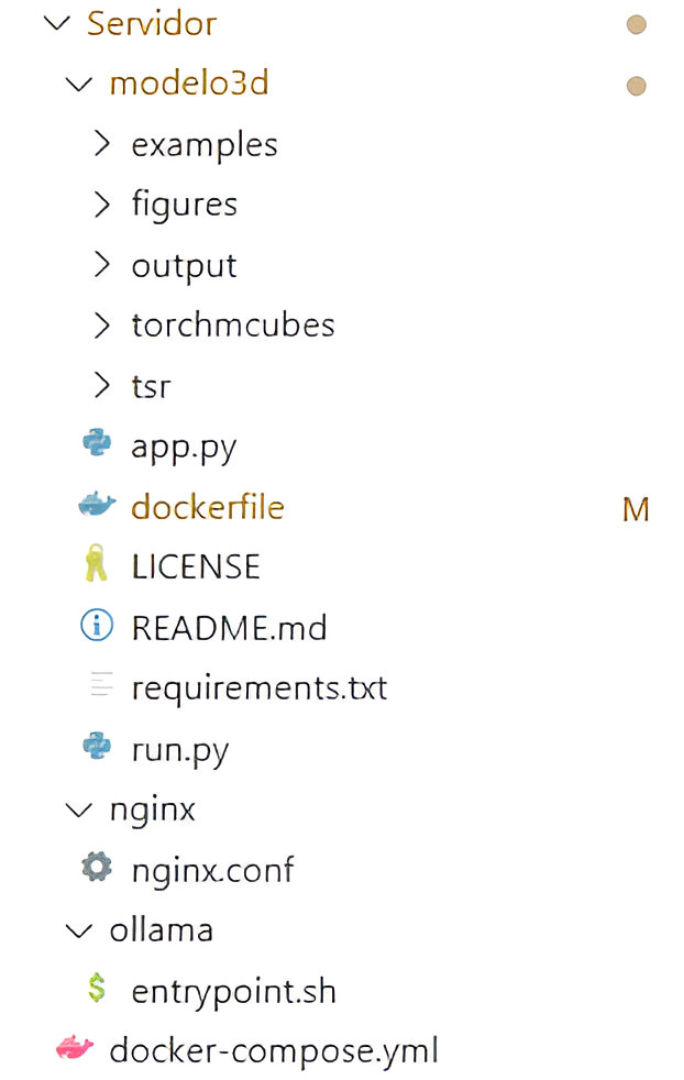
\includegraphics[width=0.4\textwidth]{figs/DistServidor.jpg}
  \caption{Distribución de las carpetas en el servidor.}
  \label{fig:carpetasServ}
\end{figure}


\newpage
\subsection{Implementación del modelo generativo LLM}
La puesta en marcha del modelo LLM Dolphin-Mistral proporcionado por Ollama se realiza mediante el script bash (\verb|entrypoint.sh|), mostrado en el Listado \ref{lst:scriptOllama}.

% % Bash
% \captionsetup{type=listing}
% \captionof{listing}{Script Bash (entrypoint.sh) de descarga e inicialización de Ollama y del modelo LLM.}
% \label{lst:scriptOllama}
% \begin{minted}[breaklines, fontsize=\small, linenos]{bash}
%     #!/bin/sh

%     # Inicia el servidor Ollama en segundo plano
%     /bin/ollama serve &

%     # Espera 20 segundos para que el servidor se inicie
%     sleep 20

%     # Verificar si el modelo está presente
%     MODEL_NAME="dolphin-mistral:7b-v2.6-dpo-laser-q4_0"
%     if ! ollama list | grep -q "$MODEL_NAME"; then
%         echo "Descargando el modelo..."

%         # Crear un lock file para evitar descargas concurrentes
%         LOCK_FILE="/root/.ollama/model_download.lock"
%         if [ ! -f "$LOCK_FILE" ]; then
%             touch "$LOCK_FILE"
%             ollama pull $MODEL_NAME
%             rm -f "$LOCK_FILE"
%         else
%             # Esperar a que otro contenedor complete la descarga
%             while [ -f "$LOCK_FILE" ]; do
%                 echo "Esperando que otro contenedor termine la descarga..."
%                 sleep 10
%             done
%         fi
%     fi

%     # Mantener el contenedor en ejecución
%     tail -f /dev/null
% \end{minted}

Este script cumple la función de inicializar de forma controlada el contenedor Docker correspondiente, dentro de una composición definida por Docker Compose. El script lanza el servidor de Ollama en segundo plano (\verb|/bin/ollama serve &|) y establece un tiempo de espera (\verb|sleep 20|) destinado a garantizar que el servicio se estabilice correctamente antes de continuar con los siguientes pasos. A continuación, el script comprueba mediante la interfaz de línea de comandos de Ollama (\verb|ollama list or grep -q "$MODEL_NAME"|) si el modelo \verb|dolphin-mistral:7b-v2.6-dpo-laser-q4-0| ya se encuentra disponible en el sistema, este modelo es la versión \verb|q4-0| menos cuantizada a la del modelo que se había planteado previamente que era \verb|dolphin-mistral:7b-v2.6-dpo-laser-q8-0| debido a que el modelo con \verb|q8-0| es uno más costoso computacionalmente y se planteo usar uno más liviano para obtener un mejor rendimiento. En caso de no detectarlo, se activa un mecanismo de control de concurrencia mediante un archivo de bloqueo (\verb|/root/.ollama/model_download.lock|). Este archivo actúa como semáforo para evitar descargas duplicadas en contextos donde múltiples contenedores podrían iniciarse de forma simultánea. Si el archivo ya existe, el contenedor entra en un bucle de espera activa hasta que el recurso quede liberado, en caso contrario, se crea el archivo, se descarga el modelo requerido (\verb|ollama pull $MODEL_NAME|) y se elimina el bloqueo una vez finalizada la operación. Este proceso está incorporado dentro del ecosistema de servicios a través de un proxy, como se ha descrito previamente, el cual redirecciona las solicitudes emitidas desde Blender hacia los contenedores que ya cuentan con el modelo preparado.


\subsection{Implementación del modelo generativo 3D}
La implementación del modelo generativo TripoSR se ha estructurado en un conjunto de componentes organizados jerárquicamente, tal como se muestra en la Figura \ref{fig:carpetasModel3D}. En primer lugar, se encuentran los directorios \verb|examples| y \verb|figures|, que contienen ejemplos ilustrativos proporcionados por el repositorio original. Estas carpetas incluyen tanto imágenes de entrada como modelos 3D de referencia generados, útiles para validar el comportamiento del modelo durante la fase de pruebas. A continuación, se destaca la carpeta \verb|output|, que tiene un papel central en el flujo de ejecución del servicio, ya que almacena el modelo tridimensional generado por el sistema. Este archivo es posteriormente devuelto al proxy y este al add-on de Blender. También se incluye el directorio correspondiente a la biblioteca \verb|torchmcubes|, la cual ha requerido modificaciones manuales en su proceso de instalación debido a problemas de compatibilidad, como se explicó previamente. La carpeta \verb|tsr| contiene los archivos compilados necesarios para la ejecución del modelo, incluyendo los pesos preentrenados y los módulos auxiliares que conforman el núcleo funcional de TripoSR. En la raíz del proyecto, se localiza el archivo \verb|app.py|, que define la API construida con Flask encargada de recibir las solicitudes, ejecutar el modelo y retornar la salida correspondiente. El entorno se completa con el archivo \verb|Dockerfile|, el cual describe las instrucciones necesarias para la construcción de la imagen del servicio 3D dentro del contenedor. Este archivo hace uso del documento \verb|requirements.txt|, que especifica las dependencias del proyecto y permite su instalación automatizada durante el proceso de build, cuyo contenido se muestra en el Listado \ref{lst:dependencias3D}. Finalmente, el archivo \verb|run.py| contiene el script principal en Python que lanza la ejecución del modelo TripoSR y coordina la generación del modelo tridimensional a partir de la imagen de entrada.

% Imagen orden carpetas modelo3d
\begin{figure}[h!tb]
  \centering
  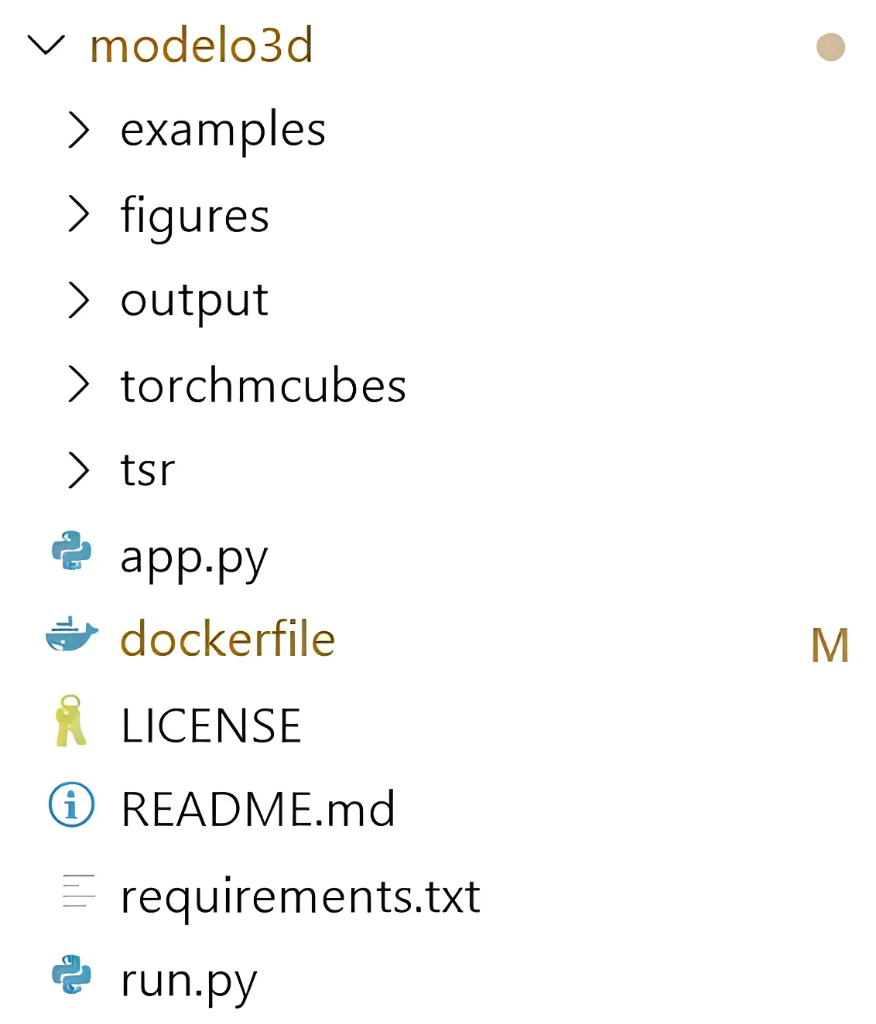
\includegraphics[width=0.4\textwidth]{figs/DistModelo3D.png}
  \caption{Distribución de las carpetas en el modelo 3D.}
  \label{fig:carpetasModel3D}
\end{figure}

% \newpage % Quitar cuando esté referenciado
% % Imagen requeriments.txt
% \captionsetup{type=listing}
% \captionof{listing}{Archivo (requirements.txt) de dependencias del modelo 3D.}
% \label{lst:dependencias3D}
% \begin{minted}[breaklines, fontsize=\small, linenos]{text}
%     flask
%     flask-cors
%     onnxruntime
%     gunicorn
%     omegaconf==2.3.0
%     Pillow==10.1.0
%     einops==0.7.0
%     transformers==4.35.0
%     trimesh==4.0.5
%     rembg
%     huggingface-hub
%     imageio[ffmpeg]
% \end{minted}

El Listado \ref{lst:appAPI3d} muestra el código de \verb|app.py| que se encarga de implementar el servicio REST para la inferencia del modelo generativo 3D TripoSR utilizando el framework Flask, actuando como mediador entre el proxy inverso Nginx y el motor de procesamiento 3D.
Los datos de entrada son gestionados a través del endpoint \verb|/upload|, el cual está configurado con el decorador \verb|@app.route('/upload', methods=['POST'])| y se utiliza para recibir archivos binarios enviados desde el add-on de Blender mediante \verb|request.files['image']|. Tras recibir la imagen, esta se pasa a la función \verb|generate_geometry(image_data)|, que se importa del script \verb|run.py|, para ejecutar el modelo TripoSR, produciendo como salida una malla en formato GLB. El archivo resultante se almacena temporalmente en el directorio \verb|output/0/|. La entrega del archivo generado al cliente se realiza mediante la función \verb|send_file(...)|, configurada con el tipo MIME \verb|model/gltf-binary| y encabezados apropiados para su correcta interpretación en Blender. Para permitir la interoperabilidad entre dominios dentro del entorno orquestado, se habilitan las políticas CORS mediante la instrucción \verb|flask_cors.CORS(app)|, lo que posibilita el acceso al servicio desde el proxy Nginx sin restricciones de origen y una simplificación del servicio a un único punto de entrada \verb|/upload|, reduciendo la complejidad estructural y minimizando la latencia. El servicio se expone en la dirección \verb|0.0.0.0| mediante \verb|app.run(host='0.0.0.0')|, lo que permite su correcta integración en el sistema de contenedores desplegado con Docker y su comunicación directa con el proxy. Por otro lado, el código Python del Listado \ref{lst:runAPI3d} es el código que ejecuta al modelo y incluye varias adaptaciones respecto al repositorio original de TripoSR, entre las cuales destaca la eliminación de la interfaz web desarrollada con Gradio, como se mencionó anteriormente.

% % Código API modelo3d
% \captionsetup{type=listing}
% \captionof{listing}{Código python (app.py) de la API Flask del modelo 3D.}
% \label{lst:appAPI3d}
% \begin{minted}[breaklines, fontsize=\small, linenos]{python}
%     from run import generate_geometry
%     from flask import Flask, request, send_file
%     from flask_cors import CORS
%     import os
%     import time

%     app = Flask(__name__)
%     CORS(app)

%     def check_file_existence(directory, filename):
%         """Function to check if a file exists in a directory."""
%         return os.path.exists(os.path.join(directory, filename))

%     @app.route('/upload', methods=['POST'])
%     def upload_file():
%         if 'image' in request.files:
%             image = request.files['image']
%             directory = 'output/0'
%             filename_mesh = 'mesh.glb'

%             # Lee los datos binarios de la imagen
%             image_data = image.read()
%             generate_geometry(image_data)  # Pasa los datos binarios

%             return send_file(os.path.join(directory, filename_mesh), as_attachment=True, mimetype='model/gltf-binary')
%         else:
%             return 'No image provided', 400

%     if __name__ == '__main__':
%         app.run(host='0.0.0.0')
% \end{minted}

% % Código modelo3d adaptado
% \captionsetup{type=listing}
% \captionof{listing}{Código python (run.py) que ejecuta el modelo 3D adaptado.}
% \label{lst:runAPI3d}
% \begin{minted}[breaklines, fontsize=\small, linenos]{python}
%     import argparse
%     import logging
%     import os
%     import time

%     import numpy as np
%     import rembg
%     import torch
%     from PIL import Image
%     from io import BytesIO

%     from tsr.system import TSR
%     from tsr.utils import remove_background, resize_foreground, save_video

%     def generate_geometry(image_web):
%         class Timer:
%             def __init__(self):
%                 self.items = {}
%                 self.time_scale = 1000.0  # ms
%                 self.time_unit = "ms"

%             def start(self, name: str) -> None:
%                 if torch.cuda.is_available():
%                     torch.cuda.synchronize()
%                 self.items[name] = time.time()
%                 logging.info(f"{name} ...")

%             def end(self, name: str) -> float:
%                 if name not in self.items:
%                     return
%                 if torch.cuda.is_available():
%                     torch.cuda.synchronize()
%                 start_time = self.items.pop(name)
%                 delta = time.time() - start_time
%                 t = delta * self.time_scale
%                 logging.info(f"{name} finished in {t:.2f}{self.time_unit}.")

%         timer = Timer()

%         logging.basicConfig(
%             format="%(asctime)s - %(levelname)s - %(message)s", level=logging.INFO
%         )

%         input_image = image_web      #"examples/chair.png"
%         output_dir = "output/"
%         device = "cuda:0"   #"cpu"
%         pretrained = "stabilityai/TripoSR"
%         chunksize = 8192
%         noremove_bg = False
%         foreground = 0.85
%         resolution = 256
%         model_format = "glb"    #"obj"
%         render_store = False

%         os.makedirs(output_dir, exist_ok=True)

%         if not torch.cuda.is_available():
%             device = "cpu"

%         timer.start("Initializing model")
%         model = TSR.from_pretrained(
%             pretrained,
%             config_name="config.yaml",
%             weight_name="model.ckpt",
%         )
%         model.renderer.set_chunk_size(chunksize)
%         model.to(device)
%         timer.end("Initializing model")

%         timer.start("Processing images")
%         images = []

%         if noremove_bg:
%             rembg_session = None
%         else:
%             rembg_session = rembg.new_session()

%         if noremove_bg:
%             image = np.array(Image.open(BytesIO(input_image)).convert("RGB"))
%         else:
%             image = remove_background(Image.open(BytesIO(input_image)), rembg_session)
%             image = resize_foreground(image, foreground)
%             image = np.array(image).astype(np.float32) / 255.0
%             image = image[:, :, :3] * image[:, :, 3:4] + (1 - image[:, :, 3:4]) * 0.5
%             image = Image.fromarray((image * 255.0).astype(np.uint8))
%             if not os.path.exists(os.path.join(output_dir, str(0))):
%                 os.makedirs(os.path.join(output_dir, str(0)))
%             image.save(os.path.join(output_dir, str(0), f"input.png"))
%         images.append(image)
%         timer.end("Processing images")

%         for i, image in enumerate(images):
%             logging.info(f"Running image {i + 1}/{len(images)} ...")

%             timer.start("Running model")
%             with torch.no_grad():
%                 scene_codes = model([image], device=device)
%             timer.end("Running model")

%             if render_store:
%                 timer.start("Rendering")
%                 render_images = model.render(scene_codes, n_views=30, return_type="pil")
%                 for ri, render_image in enumerate(render_images[0]):
%                     render_image.save(os.path.join(output_dir, str(i), f"render_{ri:03d}.png"))
%                 save_video(
%                     render_images[0], os.path.join(output_dir, str(i), f"render.mp4"), fps=30
%                 )
%                 timer.end("Rendering")

%             timer.start("Exporting mesh")
%             meshes = model.extract_mesh(scene_codes, resolution=resolution)
%             meshes[0].export(os.path.join(output_dir, str(i), f"mesh.{model_format}"))
%             timer.end("Exporting mesh")
% \end{minted}


El archivo \verb|Dockerfile| que aparece en el Listado \ref{lst:dockerfileM3D} establece una estrategia de construcción estructurada para generar una imagen personalizada del modelo TripoSR, abordando múltiples desafíos técnicos asociados al despliegue de entornos de inferencia basados en inteligencia artificial dentro de arquitecturas contenerizadas. La imagen se basa en la distribución \verb|python:3.8-slim|, seleccionada por su equilibrio entre ligereza y soporte funcional, permitiendo reducir significativamente el tamaño del contenedor sin comprometer su compatibilidad con las bibliotecas requeridas.
% \newpage
% % Dockerfile modelo3d
% \captionsetup{type=listing}
% \captionof{listing}{Dockerfile de la imagen de Docker del servicio del modelo 3D.}
% \label{lst:dockerfileM3D}
% \begin{minted}[breaklines, fontsize=\small, linenos]{dockerfile}
%     # Utiliza una imagen base de Python
%     FROM python:3.8-slim

%     # Establece el directorio de trabajo en el contenedor
%     WORKDIR /app

%     # Copia los archivos de la aplicación Flask al contenedor
%     COPY . /app

%     # Actualiza setuptools y luego instala las dependencias de Python
%     RUN pip install --upgrade setuptools && pip install -r requirements.txt && pip install torch torchvision torchaudio -f https://download.pytorch.org/whl/torch_stable.html

%     # Cambia al directorio del repositorio
%     WORKDIR /app/torchmcubes

%     RUN apt-get update && \
%         apt-get install -y g++ ninja-build && \
%         apt-get clean && \
%         rm -rf /var/lib/apt/lists/*

%     # Ejecuta el script de Python que genera la carpeta y el archivo .pyd
%     RUN python setup.py build_ext -i

%     # Mueve los archivos generados a la carpeta de librerías de Python
%     RUN mv torchmcubes /usr/local/lib/python3.8/site-packages/torchmcubes && \
%         mv build/lib.linux-x86_64-cpython-38/
%         torchmcubes_module.cpython-38-x86_64-linux-gnu.so 
%         /usr/local/lib/python3.8/site-packages/

%     WORKDIR /app

%     RUN rm -rf torchmcubes

%     # Expone el puerto en el que se ejecutará la aplicación Flask
%     EXPOSE 5000

%     # Ejecuta la aplicación Flask con Gunicorn para producción
%     CMD ["gunicorn", "-b", "0.0.0.0:5000", "--timeout", "1000", "app:app"]
% \end{minted}
El proceso de instalación de dependencias se ejecuta de manera controlada, comenzando con la actualización del gestor de paquetes \verb|setuptools|, seguida de la incorporación de las librerías especificadas en \verb|requirements.txt| y la inclusión explícita de los paquetes de PyTorch (\verb|torch|, \verb|torchvision|, \verb|torchaudio|) a través de binarios precompilados, con el objetivo de evitar compilaciones locales que incrementarían el tiempo de construcción y el tamaño de la imagen. Una parte crítica del proceso consiste en la integración manual de bibliotecas que presentan incompatibilidades documentadas, como \verb|torchmcubes|. Para solventar dichas incidencias, se incorpora una fase de compilación directa empleando herramientas del sistema (\verb|g++|, \verb|ninja-build|) y la instrucción \verb|python setup.py build_ext -i|, tras lo cual se reubica la biblioteca compilada en el directorio correspondiente de paquetes de Python, asegurando su correcto enlace durante la ejecución del modelo. Posteriormente, se lleva a cabo una fase de depuración del entorno mediante la eliminación de los archivos fuente y directorios intermedios utilizados durante la compilación, con el fin de minimizar tanto el tamaño final de la imagen como su superficie de exposición. Finalmente, el despliegue del servicio se configura para su ejecución bajo un entorno productivo utilizando el servidor WSGI Gunicorn, expuesto en la dirección \verb|0.0.0.0:5000|, y con un parámetro de espera extendido (\verb|timeout|) fijado en 1000 segundos. Esta configuración está orientada a garantizar la tolerancia a procesos computacionalmente intensivos propios de la generación 3D.




\subsection{Implementación y despliegue del servidor con Docker-Compose y Nginx}
El proceso de despliegue del servidor requiere la activación previa del entorno de ejecución Linux proporcionado por \gls{wsl2}, seguido del inicio manual del servicio Docker mediante la instrucción \verb|/etc/init.d/docker start|. Una vez iniciado el servicio, es necesario acceder al directorio del proyecto que contiene el archivo \verb|docker-compose.yml|, desde donde se ejecuta el comando \verb|docker-compose up -d --build --scale ollama=2 --scale modelo3d=2|. Este comando lanza el proceso de construcción y despliegue de los contenedores en segundo plano (\verb|-d|), fuerza la reconstrucción de las imágenes involucradas (\verb|--build|) y escala explícitamente el número de instancias del servicio \verb|ollama| y del servicio \verb|modelo3d| a dos contenedores cada uno (\verb|--scale|), permitiendo una mayor concurrencia en la atención de solicitudes por parte de los modelos de inteligencia artificial. La correcta ejecución de estas instrucciones puede observarse en las Figuras \ref{fig:despliegueServer1}, \ref{fig:despliegueServer2}, \ref{fig:despliegueServer3} y \ref{fig:despliegueServer4}, que documentan visualmente el estado del sistema tras la inicialización. Para la orquestación completa del entorno contenerizado se han utilizado, además del archivo \verb|docker-compose.yml|, los parámetros de configuración definidos en \verb|nginx.conf|, que permiten gestionar tanto el direccionamiento interno de las solicitudes como el balanceo de carga entre servicios concurrentes.

% Imagen despliegue docker
\begin{figure}[h!tb]
  \centering
  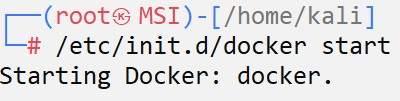
\includegraphics[width=0.3\textwidth]{figs/initDocker.jpg}
  \caption{Comando de inicio Docker en el entorno linux.}
  \label{fig:despliegueServer1}
\end{figure}

% Imagen despliegue servidor
\begin{figure}[h!tb]
  \centering
  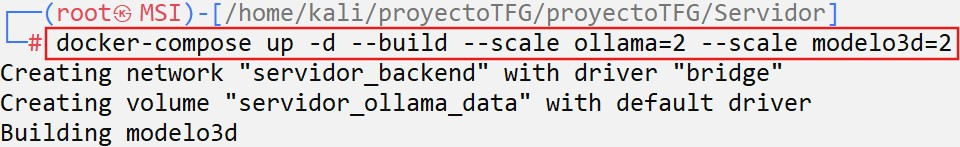
\includegraphics[width=0.7\textwidth]{figs/initServer.jpg}
  \caption{Comando de inicio Docker-Compose en el entorno linux.}
  \label{fig:despliegueServer2}
\end{figure}

% Imagen despliegue servidor
\begin{figure}[h!tb]
  \centering
  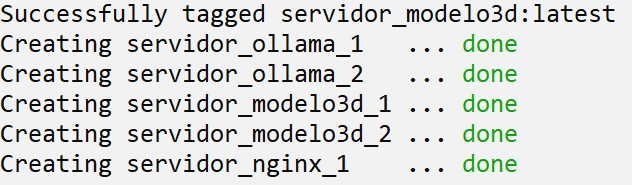
\includegraphics[width=0.5\textwidth]{figs/initServer2.jpg}
  \caption{Resultado del inicio del Docker-Compose en el entorno linux.}
  \label{fig:despliegueServer3}
\end{figure}

% Imagen despliegue servidor
\begin{figure}[h!tb]
  \centering
  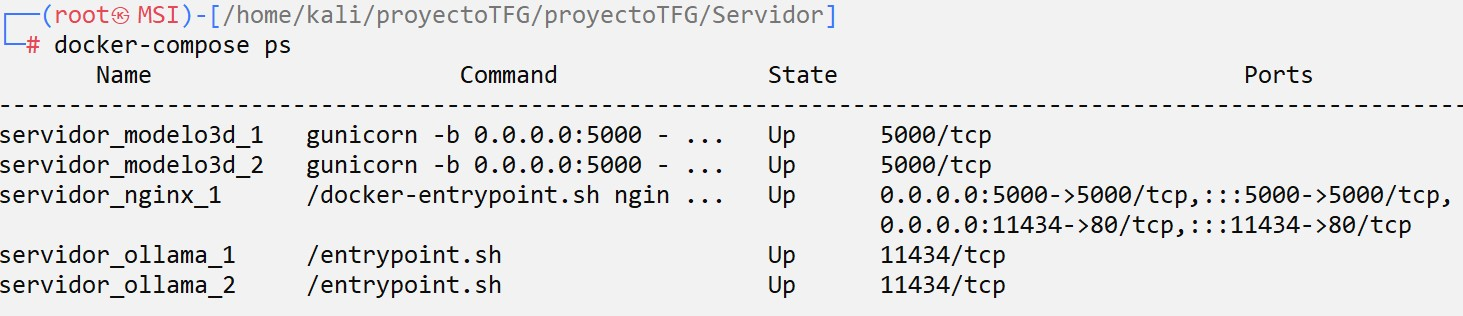
\includegraphics[width=1.0\textwidth]{figs/initServer3.jpg}
  \caption{Verificación del estado del servidor mediante docker-compose ps.}
  \label{fig:despliegueServer4}
\end{figure}


El archivo \verb|docker-compose.yml| que se muestra en el Listado \ref{lst:composeServidor} especifica la arquitectura de servicios que conforman el entorno de peticiones y sus componentes auxiliares, utilizando la versión 3.8 de la especificación de Docker Compose como base para la definición de recursos y configuraciones. Dentro de esta estructura, se declara un servicio denominado \verb|ollama|, basado en la imagen oficial \verb|ollama/ollama|, al cual se le asigna un volumen persistente denominado \verb|ollama_data|, montado en la ruta \verb|/root/.ollama|. Este volumen permite conservar tanto los modelos de lenguaje como sus metadatos, asegurando su disponibilidad entre reinicios del contenedor. El arranque del servicio se gestiona mediante un script personalizado (\verb|./ollama/entrypoint.sh|), cuyo propósito es garantizar la correcta inicialización del demonio responsable de ejecutar el modelo LLM al momento de levantar la instancia del contenedor. La red utilizada en el despliegue se define como \verb|backend|, empleando el controlador \verb|bridge| con el objetivo de aislar el tráfico de datos interno entre servicios, sin exponer directamente sus puertos al sistema anfitrión, lo que incrementa la seguridad de la infraestructura. En términos de asignación de recursos, se establecen límites y reservas de memoria específicos en la sección \verb|deploy.resources|, configurándose un límite de 4 GB para el servicio de lenguaje (LLM), lo que permite una carga eficiente de modelos de gran tamaño, y un límite de 6 GB para el modelo generativo 3D, dado el mayor consumo asociado a la reconstrucción 3D. Esta segmentación es esencial para prevenir errores de agotamiento de memoria (OOM) y mantener una ejecución estable durante el procesamiento de inferencias. Adicionalmente, el mismo archivo permite la inclusión de otros servicios, tales como servidores proxy o balanceadores de carga, cuya configuración puede ser ajustada mediante variables de entorno como \verb|NGINX_WORKER_PROCESSES=4| y asignaciones personalizadas de recursos.

% % docker-compose.yml
% \captionsetup{type=listing}
% \captionof{listing}{Archivo de configuración Docker-Compose del despliegue del servidor en local.}
% \label{lst:composeServidor}
% \begin{minted}[breaklines, fontsize=\small, linenos]{yaml}
%     version: '3.8'

%     services:
%       ollama:
%         image: ollama/ollama
%         volumes:
%           - ollama_data:/root/.ollama
%           - ./ollama/entrypoint.sh:/entrypoint.sh
%         entrypoint: /entrypoint.sh
%         networks:
%           - backend
%         deploy:
%           resources:
%             limits:
%               memory: 4G  # Más espacio para cargar modelos grandes
%             reservations:
%               memory: 1G

%       modelo3d:
%         build:
%           context: ./modelo3d
%         networks:
%           - backend
%         deploy:
%           replicas: 2
%           resources:
%             limits:
%               memory: 6G  # Más memoria para cada instancia
%             reservations:
%               memory: 3G

%       nginx:
%         image: nginx:alpine
%         ports:
%           - "11434:80"
%           - "5000:5000"
%         volumes:
%           - ./nginx/nginx.conf:/etc/nginx/nginx.conf
%         depends_on:
%           - ollama
%           - modelo3d
%         networks:
%           - backend
%         environment:
%           - NGINX_WORKER_PROCESSES=4
%         deploy:
%           resources:
%             reservations:
%               memory: 256M

%     volumes:
%       ollama_data:

%     networks:
%       backend:
%         driver: bridge
% \end{minted}


La configuración definida en el archivo \verb|nginx.conf| que se muestra en el Listado \ref{lst:nginxConfig} establece un esquema de proxy inverso orientado a la orquestación y enrutamiento eficiente de peticiones hacia los servicios internos del sistema, concretamente el modelo \gls{llm} y el generador 3D, ambos desplegados como contenedores Docker conectados a través de una red virtual. Para ello, se recurre al uso de bloques \verb|upstream| que agrupan instancias del servicio bajo los nombres \verb|ollama_servers| (dirigido a \verb|ollama:11434|) y \verb|modelo3d_servers| (dirigido a \verb|modelo3d:5000|), apoyándose en el resolver interno de Docker (\verb|127.0.0.11|) que permite balancear dinámicamente las conexiones entre contenedores en función de su disponibilidad, sin necesidad de reconfiguración manual. En el bloque \verb|events|, se establece un valor de \verb|worker_connections 1024|, dimensionado para asegurar una concurrencia adecuada bajo condiciones de carga moderada. La sección \verb|http| define dos servidores virtuales: el primero escucha en el puerto 80 y canaliza las solicitudes dirigidas a la ruta \verb|/api/generate| hacia el servicio de lenguaje \gls{llm}, configurando \verb|proxy_http_version 1.1| y cabeceras como \verb|Host| y \verb|Connection| para preservar la integridad de las comunicaciones en solicitudes mantenidas (keep-alive). Adicionalmente, se establecen parámetros de temporización extendida (\verb|proxy_connect_timeout|, \verb|proxy_send_timeout|, \verb|proxy_read_timeout|, \verb|send_timeout| con valores de hasta 900 segundos) con el fin de soportar procesos de inferencia de alta complejidad y duración prolongada sin incurrir en errores de expiración por tiempo. El segundo servidor virtual, configurado para escuchar en el puerto 5000, gestiona las solicitudes entrantes en la ruta \verb|/upload|, redirigiéndolas hacia el contenedor encargado de la reconstrucción 3D. Este bloque replica las configuraciones de proxy y temporización ya descritas, pero incorpora además la directiva \verb|client_max_body_size 100M|, que amplía el límite de carga de archivos entrantes y garantiza la aceptación de imágenes de gran tamaño, necesarias para la generación precisa de modelos 3D.

% % nginx.conf
% \captionsetup{type=listing}
% \captionof{listing}{Archivo de configuración Nginx (nginx.conf) del proxy del servidor.}
% \label{lst:nginxConfig}
% \begin{minted}[breaklines, fontsize=\small, linenos]{nginx}
%     events {
%         worker_connections 1024;
%     }

%     http {
%         # DNS de Docker para balanceo automático
%         resolver 127.0.0.11 valid=10s;

%         upstream ollama_servers {
%             server ollama:11434;
%         }

%         upstream modelo3d_servers {
%             server modelo3d:5000;
%         }

%         server {
%             listen 80;

%             location /api/generate {
%                 proxy_pass http://ollama_servers;
%                 proxy_http_version 1.1;
%                 proxy_set_header Host $host;
%                 proxy_set_header Connection '';

%                 # Timeouts extendidos
%                 proxy_connect_timeout       900;
%                 proxy_send_timeout          900;
%                 proxy_read_timeout          900;
%                 send_timeout                900;
%             }
%         }

%         server {
%             listen 5000;

%             location /upload {
%                 proxy_pass http://modelo3d_servers;
%                 proxy_http_version 1.1;
%                 proxy_set_header Host $host;
%                 proxy_set_header Connection '';
%                 client_max_body_size        100M;

%                 # Timeouts extendidos para generación 3D
%                 proxy_connect_timeout       900;
%                 proxy_send_timeout          900;
%                 proxy_read_timeout          900;
%                 send_timeout                900;
%             }
%         }
%     }
% \end{minted}



\section{Pruebas}
En esta sección se detalla el conjunto de pruebas aplicadas al sistema para verificar su correcto funcionamiento, estabilidad, eficiencia y adecuación a los requisitos definidos. En primer lugar, se presentan las pruebas unitarias, centradas en garantizar la correcta ejecución de las funciones individuales en los servicios que conforman la arquitectura. En segundo lugar, se describen las pruebas funcionales, destinadas a comprobar el cumplimiento de los requisitos establecidos en la fase de análisis, evaluando el comportamiento global del sistema frente a escenarios de uso definidos. A continuación, se abordan las pruebas de rendimiento, orientadas a analizar la capacidad del sistema para gestionar múltiples solicitudes concurrentes, midiendo métricas clave como el tiempo de respuesta, la carga máxima soportada y la estabilidad bajo estrés. Posteriormente, se incluyen pruebas de usabilidad, cuyo propósito es recoger la percepción de los usuarios finales sobre la experiencia de interacción con la aplicación, considerando aspectos como la claridad de la interfaz, la facilidad de uso y la satisfacción general. Finalmente, se detallan las pruebas de seguridad, dirigidas a evaluar la resiliencia del sistema frente a vulnerabilidades potenciales, con el fin de comprobar la robustez de los servicios desplegados.

\subsection{Pruebas unitarias de servicios}
En esta subsección se llevarán a cabo pruebas enfocadas en verificar el funcionamiento de cada microservicio desarrollado. El primero en ser evaluado es el microservicio encargado de generar código Python utilizando el modelo \gls{llm} proporcionado por Dolphin-Mistral y Ollama. Para efectuar esta prueba, se ha realizado una solicitud POST mediante el software llamado Postman \cite{PostmanWorldsLeading} a la dirección del contenedor de Ollama, específicamente al puerto 11434 y a la terminación de la API \verb|/api/generate|, donde está alojado el contenedor Docker de este microservicio. La Figura \ref{fig:resUni1} muestra cómo la solicitud retorna un JSON, el cual representa la respuesta del modelo \gls{llm} al prompt enviado.

% Imagen U1
\begin{figure}[h!tb]
  \centering
  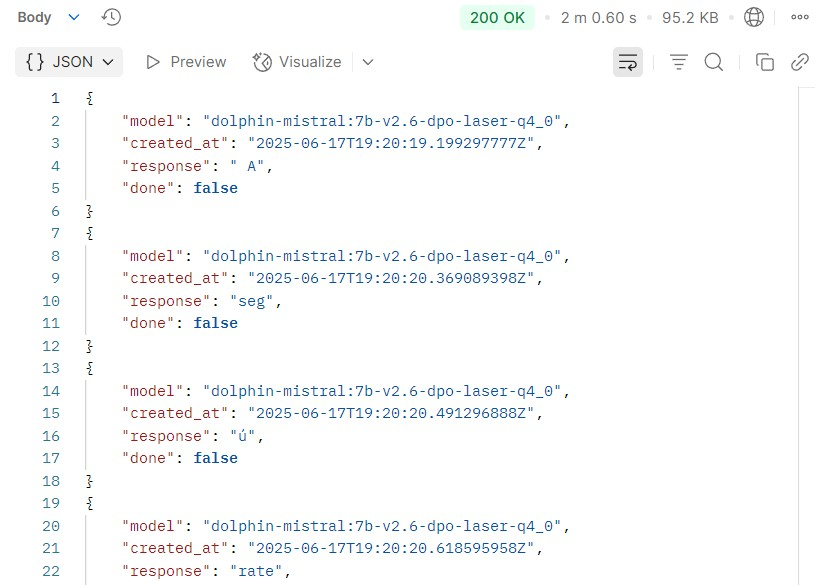
\includegraphics[width=0.8\textwidth]{figs/resUni1.jpg}
  \caption{Resultado de la prueba unitaria sobre el microservicio del modelo LLM}
  \label{fig:resUni1}
\end{figure}

El segundo y último microservicio en ser evaluado es el encargado de generar el modelo 3D a partir de una imagen utilizando el modelo OpenSource de TripoSR. Para efectuar esta prueba, se ha realizado una solicitud POST mediante el software llamado Postman a la dirección del contenedor de TripoSR, específicamente al puerto 5000 y a la terminación de la API \verb|/upload|, donde está alojado el contenedor Docker de este microservicio. La Figura \ref{fig:resUni2} muestra cómo la solicitud retorna un archivo .glb, el cual representa el modelo 3D generado a partir de la imagen de entrada.

% Imagen U2
\begin{figure}[h!tb]
  \centering
  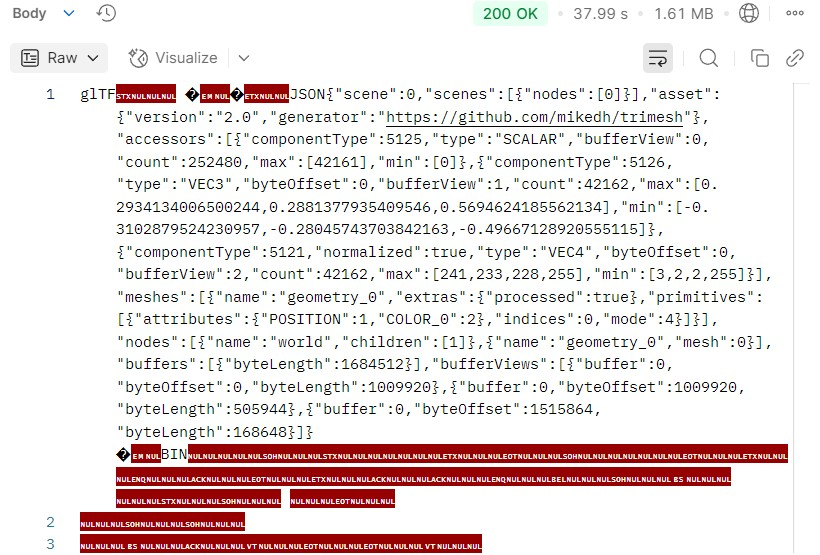
\includegraphics[width=0.8\textwidth]{figs/resUni2.jpg}
  \caption{Resultado de la prueba unitaria sobre el microservicio del modelo TripoSR}
  \label{fig:resUni2}
\end{figure}



\subsection{Pruebas funcionales}
En esta subsección se van a realizar pruebas para comprobar la funcionalidad de cada caso de uso del sistema. La Tabla \ref{tab:pruebasFuncionales}
\begin{table}[h!tb]% Tabla de las pruebas funcionales del sistema
  \centering
  \begin{adjustbox}{max width=0.9\textwidth}
    \begin{tabular}{|p{4cm}|p{4cm}|p{4cm}|p{4cm}|p{2cm}|}
      \hline
      \textbf{Caso de uso}                & \textbf{Prerrequisitos}                                                     & \textbf{Prueba}                                                                                                                                             & \textbf{Resultado esperado}                                                                                                             & \textbf{Figuras}                                   \\ \hline

      CU1:Generar Código Python           & Se debe escribir un prompt de entrada en el Add-on.                         & Realizar la petición de generar código Python.                                                                                                              & Verificar en el terminal del servidor que la solicitud para generar el código Python se lleva a cabo de manera adecuada.                & \ref{fig:cu1cu8}                                   \\ \hline

      CU2:Visualizar Resultado en Blender & Se debe haber obtenido una respuesta del modelo LLM.                        & Ingresar al campo de respuesta del modelo LLM del add-on y proceder a ejecutar el código generado utilizando el botón de ejecución de código.               & Verificar que en el campo de respuesta del modelo LLM está el código y que se ejecuta correctamente.                                    & \ref{fig:cu2_1}, \ref{fig:cu2_2} y \ref{fig:cu2_3} \\ \hline

      CU3:Cargar Imagen                   & Se debe introducir una imagen en el add-on.                                 & Ingresar en la barra de notificaciones de Blender.                                                                                                          & Comprobar en la barra de notificaciones de Blender que se ha cargado correctamente la imagen.                                           & \ref{fig:cu3}                                      \\ \hline

      CU4:Generar Modelo 3D               & Se debe importar una imagen en el add-on.                                   & Realizar la petición de generar el Modelo 3D.                                                                                                               & Verificar en el terminal del servidor que la solicitud para generar el Modelo 3D se lleva a cabo de manera adecuada.                    & \ref{fig:cu4cu9}                                   \\ \hline

      CU5:Cargar modelo 3D en Blender     & Se debe haber obtenido una respuesta del modelo generativo 3D.              & Ingresar al campo de respuesta del modelo generativo 3D del add-on y proceder a cargar el modelo 3D en Blender utilizando el botón de cargar modelo 3D.     & Verificar que en el campo de respuesta del modelo generativo 3D está el modelo 3D y que se carga correctamente en la escena de Blender. & \ref{fig:cu5_1} y \ref{fig:cu5_2}                  \\ \hline

      CU6:Exportar Modelo 3D              & Se debe haber obtenido una respuesta del modelo generativo 3D.              & Ingresar al campo de respuesta del modelo generativo 3D del add-on y proceder a exportar el modelo 3D en Blender utilizando el botón de exportar modelo 3D. & Verificar que se ha exportado correctamente el modelo 3D.                                                                               & \ref{fig:cu6_1} y \ref{fig:cu6_2}                  \\ \hline

      CU7:Deshacer Cambios                & Se debe haber realizado una acción con el add-on en Blender.                & Revertir una acción mediante Ctrl+Z.                                                                                                                        & Verificar en el terminal de Blender que se ha revertido la acción correctamente.                                                        & \ref{fig:cu7}                                      \\ \hline

      CU8:Ejecutar Modelo LLM             & Se debe haber recibido la petición de generar código python en el servidor. & Ingresar al registro de logs de los modelos LLM en el servidor.                                                                                             & Comprobar que se ejecuta el modelo LLM y que devuelve correctamente la respuesta al add-on.                                             & \ref{fig:cu1cu8}                                   \\ \hline

      CU9:Ejecutar Modelo Generativo 3D   & Se debe haber recibido la petición de generar el Modelo 3D en el servidor.  & Ingresar al registro de logs de los modelos generativos 3D en el servidor.                                                                                  & Comprobar que se ejecuta el modelo generativo 3D y que devuelve correctamente la respuesta al add-on.                                   & \ref{fig:cu4cu9}                                   \\ \hline
    \end{tabular}
  \end{adjustbox}
  \caption{Tabla con las pruebas funcionales del sistema}
  \label{tab:pruebasFuncionales}
\end{table}
muestra los casos de uso junto con los requisitos previos, los pasos requeridos para llevar a cabo las pruebas y los resultados que se anticipan.
A continuación, se procederá a realizar todas las pruebas mencionadas antes, incluyendo capturas de pantalla o listados de logs que evidencien que los resultados anticipados se cumplen. Estos resultados se registran en el Apéndice \ref{sec:puntoB1} para cada caso de uso dentro del sistema.

% \begin{itemize}
%     \item \textbf{CU1 y CU8:} La Figura \ref{fig:cu1cu8} muestra los resultados alcanzados.

%     \item \textbf{CU2:} La Figura \ref{fig:cu2_1}, \ref{fig:cu2_2} y \ref{fig:cu2_3} muestra los resultados alcanzados.

%     \item \textbf{CU3:} La Figura \ref{fig:cu3} muestra los resultados alcanzados.

%     \item \textbf{CU4 y CU9:} La Figura \ref{fig:cu4cu9} muestra los resultados alcanzados.

%     \item \textbf{CU5:} La Figura \ref{fig:cu5_1} y \ref{fig:cu5_2} muestra los resultados alcanzados.

%     \item \textbf{CU6:} La Figura \ref{fig:cu6_1} y \ref{fig:cu6_2} muestra los resultados alcanzados.

%     \item \textbf{CU7:} La Figura \ref{fig:cu7} muestra los resultados alcanzados.
% \end{itemize}


\subsection{Pruebas de rendimiento}
Las pruebas de rendimiento descritas en esta subsección tienen como finalidad evaluar la capacidad del sistema para mantener un funcionamiento estable bajo condiciones de alta demanda concurrente. El objetivo es obtener métricas clave como el tiempo medio de respuesta y el comportamiento del sistema ante situaciones de estrés. Para su ejecución, se ha diseñado un conjunto de experimentos consistentes en el envío de solicitudes simultáneas a los modelos de IA integrados (modelo LLM y modelo generativo 3D), simulando mediante el software de Postman las peticiones de los múltiples dispositivos. La carga generada se incrementa progresivamente, comenzando con una única petición dirigida a cada modelo y alcanzando hasta cuatro peticiones simultáneas por tipo de modelo. Este límite ha sido definido teniendo en cuenta las restricciones del entorno de pruebas, que se ejecuta sobre un hardware limitado y con recursos computacionales reducidos, donde el servidor ha sido desplegado con dos instancias por modelo de \gls{ia}, por lo que cuatro solicitudes concurrentes equivalen a una carga del 200\%, superando intencionadamente la capacidad nominal para observar el comportamiento bajo saturación. Dado que los dispositivos desde los cuales se emiten las peticiones son externos a la red local del servidor, ha sido necesario utilizar un mecanismo de acceso remoto a los servicios expuestos localmente. Para ello, se ha empleado la herramienta Postman, que permite la creación personalizada de peticiones, la automatización de las mismas y brinda estadísticas de cada petición y respuesta. Por otro lado, para medir el consumo y estrés del sistema en las diferentes pruebas se ha empleado la herramienta de htop en la máquina virtual del servidor, que permite visualizar el consumo de todos los núcleos de la CPU, de la memoria RAM, de la memoria Swap y visualizar el consumo de cada tarea.

Tras la ejecución de las pruebas de rendimiento, se ha observado un comportamiento progresivo en el consumo de recursos del sistema asociado al modelo de lenguaje LLM. Tal como se muestra en la Figura \ref{fig:resRend1LLM}, correspondiente a una única petición simultánea, el sistema presenta un uso medio de CPU del 74,7 \% y un consumo de memoria del 25,6 \%, sin llegar a utilizar ningún núcleo de procesamiento de forma completa y manteniéndose recursos disponibles para otras operaciones concurrentes.
% % Imagen R1
%   \begin{figure}[h!tb]
%     \centering
%     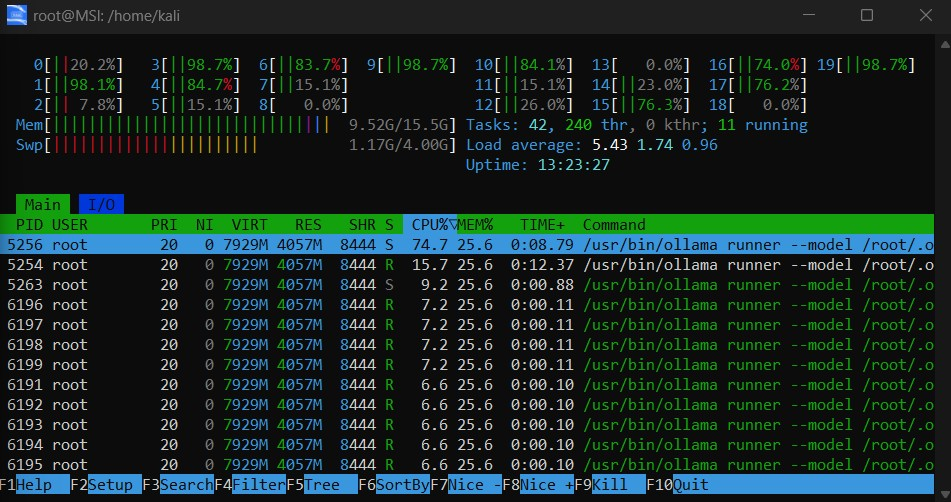
\includegraphics[width=0.8\textwidth]{figs/LLM1.jpg}
%     \caption{Resultado de la prueba de rendimiento con 1 petición sobre el microservicio del modelo LLM}
%     \label{fig:resRend1LLM}
%   \end{figure}

No obstante, al incrementar la carga con múltiples peticiones simultáneas, se evidencia un aumento significativo en la utilización de la CPU, como se ilustra en las Figuras \ref{fig:resRend2LLM} y \ref{fig:resRend3LLM}, alcanzando en el caso de cuatro solicitudes concurrentes un valor ligeramente superior al 100 \% de 100,5 \% de uso de CPU, mientras que el uso de memoria permanece estable en torno al 25,4 \%, esto último se puede observar en la Figura \ref{fig:resRend4LLM}.

% % Imagen R2
%   \begin{figure}[h!tb]
%     \centering
%     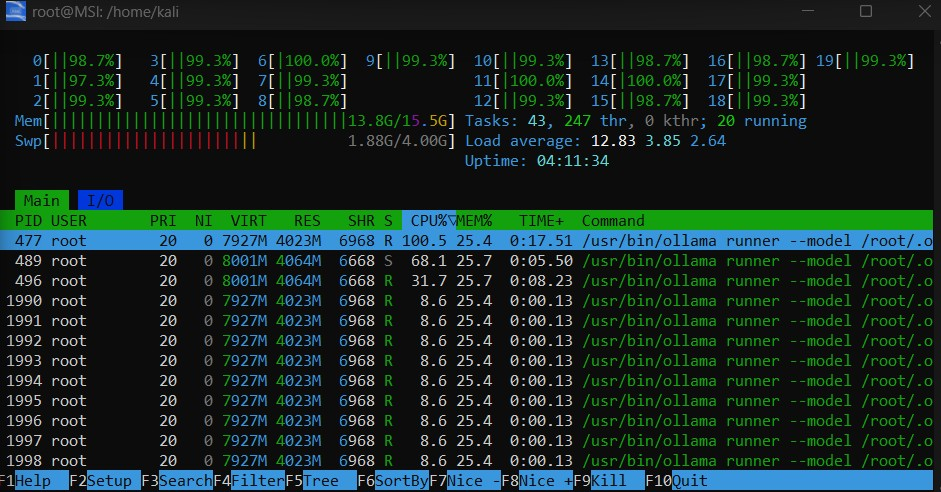
\includegraphics[width=0.8\textwidth]{figs/LLM4.jpg}
%     \caption{Resultado de la prueba de rendimiento con 4 petición sobre el microservicio del modelo LLM}
%     \label{fig:resRend4LLM}
%   \end{figure}

Este incremento en la demanda de recursos impacta directamente en la latencia de la última solicitud procesada, la cual experimenta un retraso derivado de la espera por disponibilidad de recursos computacionales y contenedores con el modelo LLM disponibles. Cabe destacar que, de acuerdo con los resultados presentados en la Tabla \ref{tab:pruebasRendimiento}, el modelo LLM presenta tiempos de respuesta superiores respecto al modelo generativo 3D, siendo el componente más lento en condiciones de carga equivalente. Esta diferencia operativa motivó la implementación del mecanismo de streaming en las respuestas del modelo LLM, permitiendo que, a pesar de una latencia total mayor, las primeras porciones de salida sean entregadas al usuario antes que en el caso del modelo generativo 3D, optimizando así la percepción de fluidez en la interacción.

% Tabla de las pruebas de usabilidad 2
\begin{table}[h!tb]
  \centering
  \begin{adjustbox}{max width=\textwidth}
    \begin{tabular}{|>{\centering\arraybackslash}p{4cm}|>{\centering\arraybackslash}p{4cm}|>{\centering\arraybackslash}p{4cm}|>{\centering\arraybackslash}p{4cm}|>{\centering\arraybackslash}p{4cm}|}
      \hline
      \textbf{Servicio}   & \textbf{Tiempo máximo (1 petición)} & \textbf{Tiempo máximo (2 petición)} & \textbf{Tiempo máximo (3 petición)} & \textbf{Tiempo máximo (4 petición)} \\ \hline

      Modelo LLM (Ollama) & 1 m 36.90 s                         & 3 m 0.30 s                          & 3 m 44.34 s                         & 3 m 50.12 s                         \\ \hline

      Modelo 3D (TripoSR) & 40.73 s                             & 1 m 23.34 s                         & 1 m 51.30 s                         & 2 m 30.12 s                         \\ \hline
    \end{tabular}
  \end{adjustbox}
  \caption{Tabla de tiempo de espera máxima por petición asociada a cada modelo de IA}
  \label{tab:pruebasRendimiento}
\end{table}


La Figura \ref{fig:resRend13D} presenta los resultados del análisis de rendimiento correspondiente a una única petición simultánea dirigida al modelo generativo 3D.
% % Imagen R3
%   \begin{figure}[h!tb]
%     \centering
%     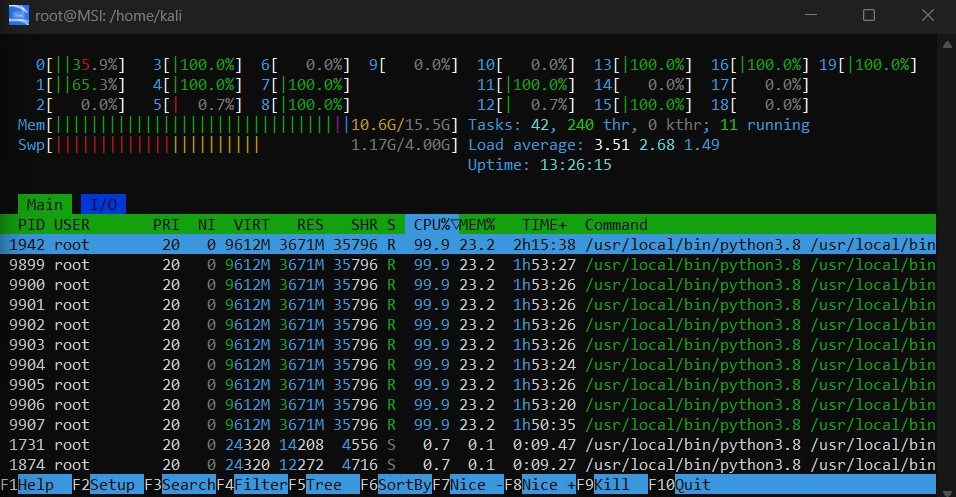
\includegraphics[width=0.8\textwidth]{figs/3D1.jpg}
%     \caption{Resultado de la prueba de rendimiento con 1 petición sobre el microservicio del modelo 3D TripoSR}
%     \label{fig:resRend13D}
%   \end{figure}
En ella se observa una utilización media de CPU del 99,9 \% y un consumo de memoria del 23,2 \%, haciendo uso intensivo de la mayoría de núcleos disponibles en el procesador. A medida que se incrementa la carga del sistema mediante múltiples solicitudes concurrentes, se constata un aumento aún más acusado en el uso de CPU en comparación con el modelo LLM, tal como se evidencia en las Figuras \ref{fig:resRend23D} y \ref{fig:resRend33D}. En el escenario con cuatro peticiones simultáneas de la Figura \ref{fig:resRend43D}, la carga computacional alcanza un valor de 100,7 \%, lo que sugiere una saturación prácticamente total de los recursos de procesamiento, mientras que la memoria RAM se mantiene relativamente estable, con un promedio de uso en torno al 24,7 \%. Este aumento en la demanda de recursos afecta directamente a la latencia observada en la última petición en ser atendida, debido a la necesidad de esperar la liberación de núcleos o la disponibilidad de instancias del contenedor del modelo 3D para poder procesarla. Es importante señalar que, según los datos recopilados, a partir de dos solicitudes concurrentes ya se produce una ocupación completa de los núcleos del procesador, lo que pone de manifiesto el elevado coste computacional asociado a la ejecución del modelo TripoSR en un hardware limitado.

% % Imagen R4
%   \begin{figure}[h!tb]
%     \centering
%     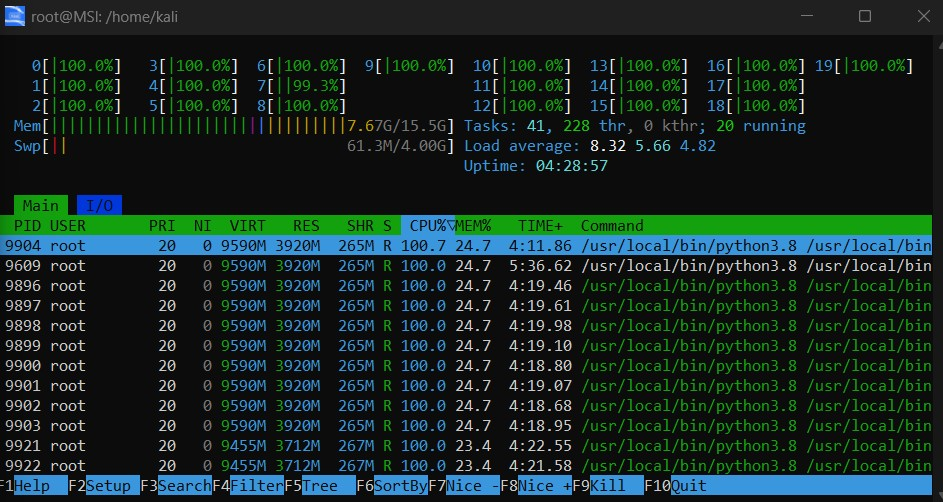
\includegraphics[width=0.8\textwidth]{figs/3D4.jpg}
%     \caption{Resultado de la prueba de rendimiento con 4 petición sobre el microservicio del modelo 3D TripoSR}
%     \label{fig:resRend43D}
%   \end{figure}



\subsection{Pruebas de usabilidad}
En esta subsección se va a evaluar la calidad percibida en términos de facilidad de uso del complemento desarrollado para Blender, se ha adoptado como instrumento de análisis el método \gls{sus}. Este procedimiento es ampliamente reconocido en el ámbito de la evaluación de interfaces de usuario por su simplicidad, fiabilidad y aplicabilidad transversal a distintos tipos de sistemas interactivos. El cuestionario está compuesto por diez afirmaciones (ver Tabla \ref{tab:preguntasSUS}) que deben ser valoradas por los usuarios empleando una escala de tipo Likert de cinco puntos, donde 1 corresponde a “totalmente en desacuerdo” y 5 a “totalmente de acuerdo”. Las afirmaciones se estructuran alternando enunciados de formulación positiva y negativa, lo que permite mitigar sesgos de respuesta y obtener una valoración más equilibrada de la experiencia de uso. El instrumento está diseñado de forma genérica, permitiendo su aplicación en una amplia variedad de entornos tecnológicos y facilitando la comparación entre soluciones de distinta naturaleza. El cálculo de la puntuación total se realiza mediante una transformación lineal, en el caso de los ítems con redacción positiva (ítems impares), se resta 1 al valor proporcionado por el usuario/a, para los ítems negativos (ítems pares), se resta la puntuación a 5. La suma de los valores transformados (en un rango de 0 a 40) se multiplica por un factor de 2.5, obteniéndose así una puntuación final normalizada en una escala de 0 a 100. Según los estándares investigados, una puntuación cercana a 68 se considera indicativa de una usabilidad media, valores superiores a 80 reflejan una percepción de alta usabilidad, mientras que resultados por debajo de 50 revelan deficiencias significativas en la experiencia de uso. En el marco del presente trabajo, este método ha sido aplicado a una muestra de usuarios que interactuaron con el add-on diseñado para Blender. La finalidad ha sido obtener una valoración cuantitativa objetiva sobre la facilidad de uso, el grado de integración funcional y la curva de aprendizaje percibida del sistema, con el fin de identificar posibles áreas de mejora en futuras iteraciones del desarrollo.\\

% Tabla de las pruebas de usabilidad 2
\begin{table}[h!tb]
  \centering
  \begin{adjustbox}{max width=\textwidth}
    \begin{tabular}{|>{\centering\arraybackslash}p{2cm}|>{\centering\arraybackslash}p{10cm}|}
      \hline
      \textbf{Número} & \textbf{Pregunta}                                                \\ \hline

      Q1              & ¿Me gustaría usarlo con frecuencia?                              \\ \hline

      Q2              & ¿Lo encontré innecesariamente complejo?                          \\ \hline

      Q3              & ¿Lo encontré fácil de usar?                                      \\ \hline

      Q4              & ¿Pensé que haría falta mucha ayuda para usarlo?                  \\ \hline

      Q5              & ¿Las funciones estaban bien integradas?                          \\ \hline

      Q6              & ¿Encontré demasiada inconsistencia en el sistema?                \\ \hline

      Q7              & ¿Imagino que la mayoría aprendería a usarlo muy rápidamente?     \\ \hline

      Q8              & ¿Encontré el sistema difícil de usar?                            \\ \hline

      Q9              & ¿Me sentí muy confiado usándolo?                                 \\ \hline

      Q10             & ¿Necesité aprender muchas cosas antes de poder funcionar con él? \\ \hline
    \end{tabular}
  \end{adjustbox}
  \caption{Tabla de preguntas del método SUS}
  \label{tab:preguntasSUS}
\end{table}

% \textbf{Componentes del SUS:}
% \begin{enumerate}
%     \item Me gustaría usarlo con frecuencia.
%     \item Lo encontré innecesariamente complejo.
%     \item Lo encontré fácil de usar.
%     \item Pensé que haría falta mucha ayuda para usarlo.
%     \item Las funciones estaban bien integradas.
%     \item Encontré demasiada inconsistencia en el sistema.
%     \item Imagino que la mayoría aprendería a usarlo muy rápidamente.
%     \item Encontré el sistema difícil de usar.
%     \item Me sentí muy confiado usándolo.
%     \item Necesité aprender muchas cosas antes de poder funcionar con él.
% \end{enumerate}

El análisis estadístico de las puntuaciones obtenidas mediante la aplicación del cuestionario SUS en las Tablas \ref{tab:pruebasUsabilidad1} y \ref{tab:pruebasUsabilidad2} revela una alta valoración general de la usabilidad del sistema, con una media aritmética de 89.3 sobre 100 y una desviación estándar de 2.9. Estos resultados reflejan una percepción homogénea por parte de los usuarios, respaldada por un coeficiente de variación del 3.25 \%, lo que indica una baja dispersión relativa respecto a la media. El rango de puntuaciones registrado, comprendido entre 85.0 y 92.5, refuerza la estabilidad de las evaluaciones y la consistencia en la experiencia de uso reportada. Cabe destacar que la totalidad de las respuestas se sitúan por encima del umbral de 80.3 que define una experiencia bastante buena en términos de usabilidad.

% Tabla de las pruebas de usabilidad 1
\begin{table}[h!tb]
  \centering
  \begin{adjustbox}{max width=\textwidth}
    \begin{tabular}{|>{\centering\arraybackslash}p{3cm}|>{\centering\arraybackslash}p{1cm}|>{\centering\arraybackslash}p{1cm}|>{\centering\arraybackslash}p{1cm}|>{\centering\arraybackslash}p{1cm}|>{\centering\arraybackslash}p{1cm}|>{\centering\arraybackslash}p{1cm}|>{\centering\arraybackslash}p{1cm}|>{\centering\arraybackslash}p{1cm}|>{\centering\arraybackslash}p{1cm}|>{\centering\arraybackslash}p{1cm}|>{\centering\arraybackslash}p{2cm}|}
      \hline
      \textbf{Participante} & \textbf{Q1} & \textbf{Q2} & \textbf{Q3} & \textbf{Q4} & \textbf{Q5} & \textbf{Q6} & \textbf{Q7} & \textbf{Q8} & \textbf{Q9} & \textbf{Q10} & \textbf{SUS (0-100)} \\ \hline

      1                     & 4           & 5           & 4           & 5           & 5           & 4           & 5           & 4           & 5           & 5            & 92.5                 \\ \hline

      2                     & 5           & 4           & 5           & 4           & 4           & 5           & 4           & 5           & 4           & 4            & 85.0                 \\ \hline

      3                     & 4           & 5           & 4           & 5           & 5           & 4           & 5           & 4           & 5           & 4            & 90.0                 \\ \hline

      4                     & 5           & 4           & 5           & 4           & 4           & 5           & 4           & 5           & 5           & 5            & 87.5                 \\ \hline

      5                     & 4           & 5           & 4           & 5           & 5           & 4           & 5           & 4           & 4           & 5            & 90.0                 \\ \hline

      6                     & 5           & 4           & 5           & 4           & 5           & 5           & 4           & 5           & 5           & 4            & 87.5                 \\ \hline

      7                     & 4           & 5           & 4           & 5           & 4           & 5           & 5           & 4           & 5           & 5            & 92.5                 \\ \hline
    \end{tabular}
  \end{adjustbox}
  \caption{Tabla de puntuaciones SUS para las pruebas de usabilidad}
  \label{tab:pruebasUsabilidad1}
\end{table}

% Tabla de las pruebas de usabilidad 2
\begin{table}[h!tb]
  \centering
  \begin{adjustbox}{max width=\textwidth}
    \begin{tabular}{|>{\centering\arraybackslash}p{4cm}|>{\centering\arraybackslash}p{4cm}|}
      \hline
      \textbf{Métrica}    & \textbf{Valor} \\ \hline

      Promedio SUS        & 89.3           \\ \hline

      Mínimo SUS          & 85.0           \\ \hline

      Máximo SUS          & 92.5           \\ \hline

      Desviación Estándar & 2.9            \\ \hline
    \end{tabular}
  \end{adjustbox}
  \caption{Tabla de los valores promedio de las puntuaciones SUS correspondientes a las pruebas de usabilidad}
  \label{tab:pruebasUsabilidad2}
\end{table}



\subsection{Pruebas de seguridad}
Esta última subsección tiene como propósito analizar el nivel de seguridad del sistema implementado, identificando posibles vulnerabilidades mediante técnicas de escaneo automatizado. Para ello, se ha utilizado la herramienta \gls{zap} \cite{ZAPHomepage}, desarrollada por OWASP y ampliamente reconocida en el ámbito de la ciberseguridad, que permite realizar análisis activos sobre aplicaciones web evaluando el comportamiento de endpoints y URLs frente a múltiples vectores de ataque. En el contexto de este proyecto, se ha empleado ZAP para someter a análisis los dos servicios expuestos del servidor de inteligencia artificial, el modelo de lenguaje LLM, accesible mediante el endpoint \verb|http://127.0.0.1:11434/api/generate| y el modelo generativo 3D, ubicado en \verb|http://127.0.0.1:5000/upload|.\\

En el primer caso, correspondiente al modelo LLM, los resultados del escaneo activo mostrados en la Figura \ref{fig:secLLM}
% Imagen S1
\begin{figure}[h!tb]
  \centering
  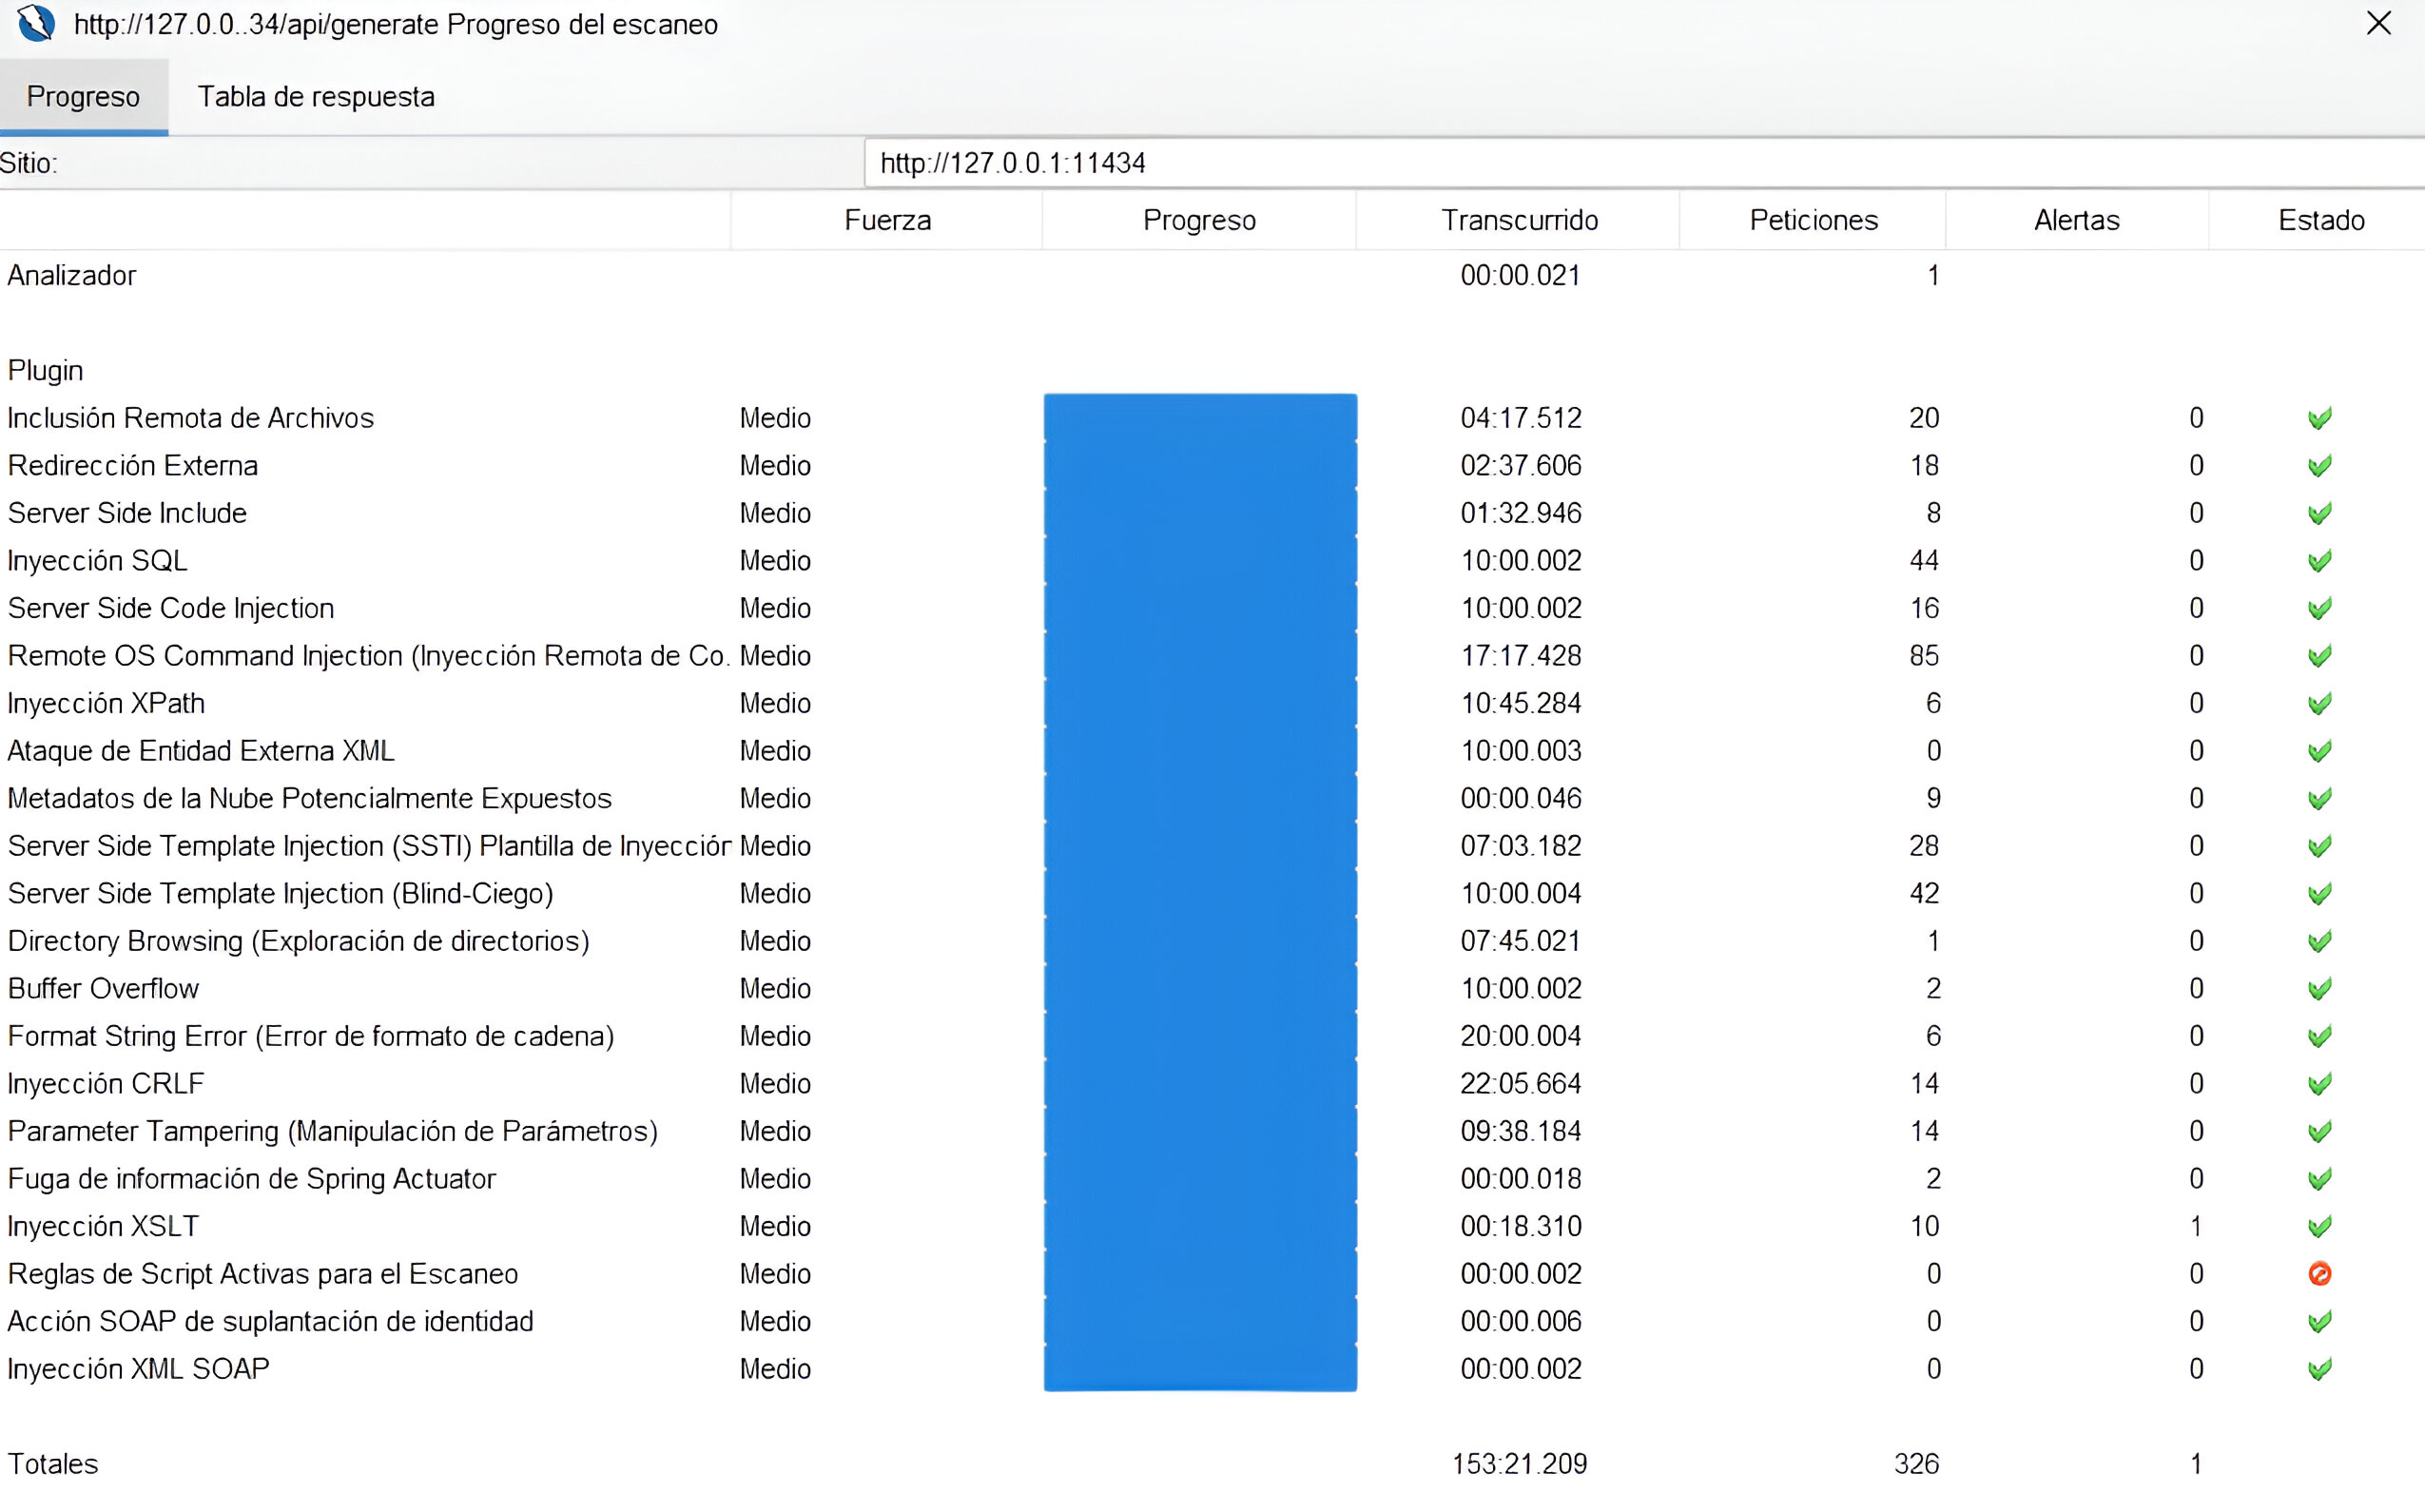
\includegraphics[width=1.0\textwidth]{figs/secLLM.jpg}
  \caption{Resultado de la prueba de seguridad sobre el endpoint del modelo LLM del servidor}
  \label{fig:secLLM}
\end{figure}
indican que la mayoría de las pruebas de seguridad fueron superadas satisfactoriamente, con excepción de las reglas asociadas a la ejecución de scripts, que no se encontraban configuradas.
No obstante, se identificó una alerta de severidad media relacionada con una posible inyección XSLT, asociada al CWE-91. El test realizado por ZAP incluyó el uso del payload \verb|xsl:value-of select="system-property('xsl vendor')"| y, como respuesta, el servidor devolvió la cadena \verb|"Microsoft"|, lo cual fue interpretado como un indicio de vulnerabilidad, tal como se muestra en la Figura \ref{fig:secVuln1}.

% Imagen S3
\begin{figure}[h!tb]
  \centering
  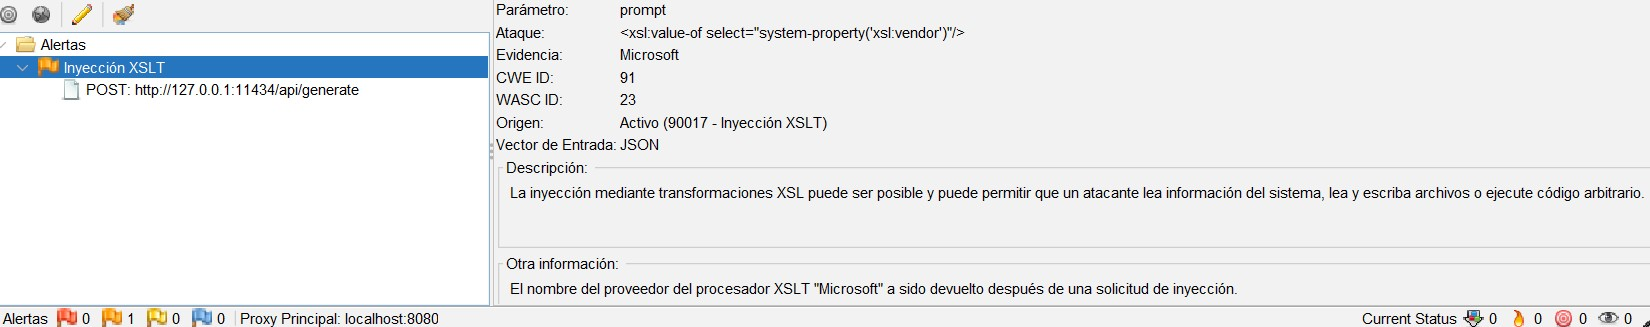
\includegraphics[width=1.0\textwidth]{figs/secVuln1.jpg}
  \caption{Vulnerabilidades obtenidas en el modelo LLM}
  \label{fig:secVuln1}
\end{figure}

Sin embargo, tras un análisis detallado del flujo de salida, representado en la Figura \ref{fig:secVuln2}, se comprobó que dicha respuesta no era resultado de una ejecución arbitraria, sino que coincidía con un fragmento generado por el propio modelo \gls{llm} en modo streaming, siendo “Microsoft” simplemente parte del contenido textual generado por el modelo en respuesta al prompt.
Esta interpretación se refuerza por el hecho de que el sistema operativo subyacente sobre el que se ejecuta el servidor es Linux, descartando así la hipótesis de una fuga real de información a través del subsistema XSLT.

% Imagen S4
\begin{figure}[h!tb]
  \centering
  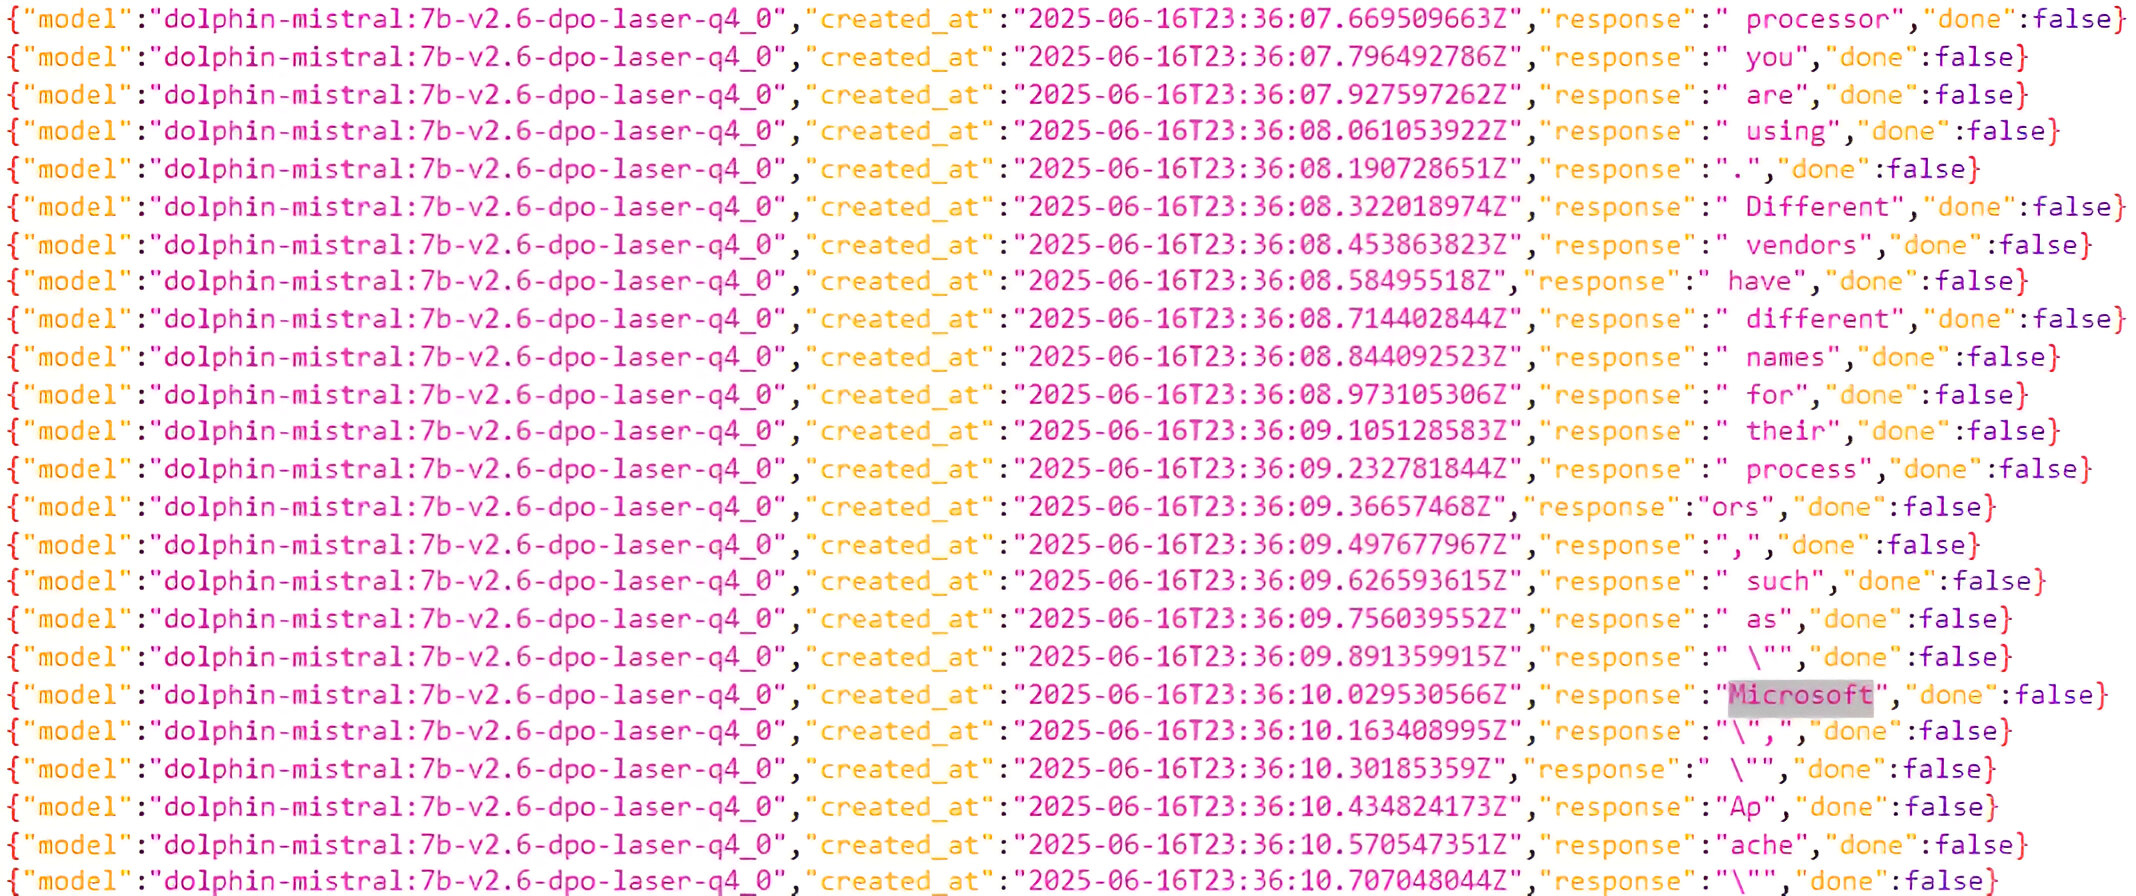
\includegraphics[width=1.0\textwidth]{figs/secVuln2.jpg}
  \caption{Detalles de la vulnerabilidad encontrada en el modelo LLM}
  \label{fig:secVuln2}
\end{figure}

En el segundo caso, correspondiente al endpoint del modelo 3D, el análisis de seguridad, consulte la Figura \ref{fig:sec3D}, mostró resultados similares y reportó también una alerta de alta severidad relacionada con una posible inyección remota de comandos (CWE-78).
% Imagen S2
\begin{figure}[h!tb]
  \centering
  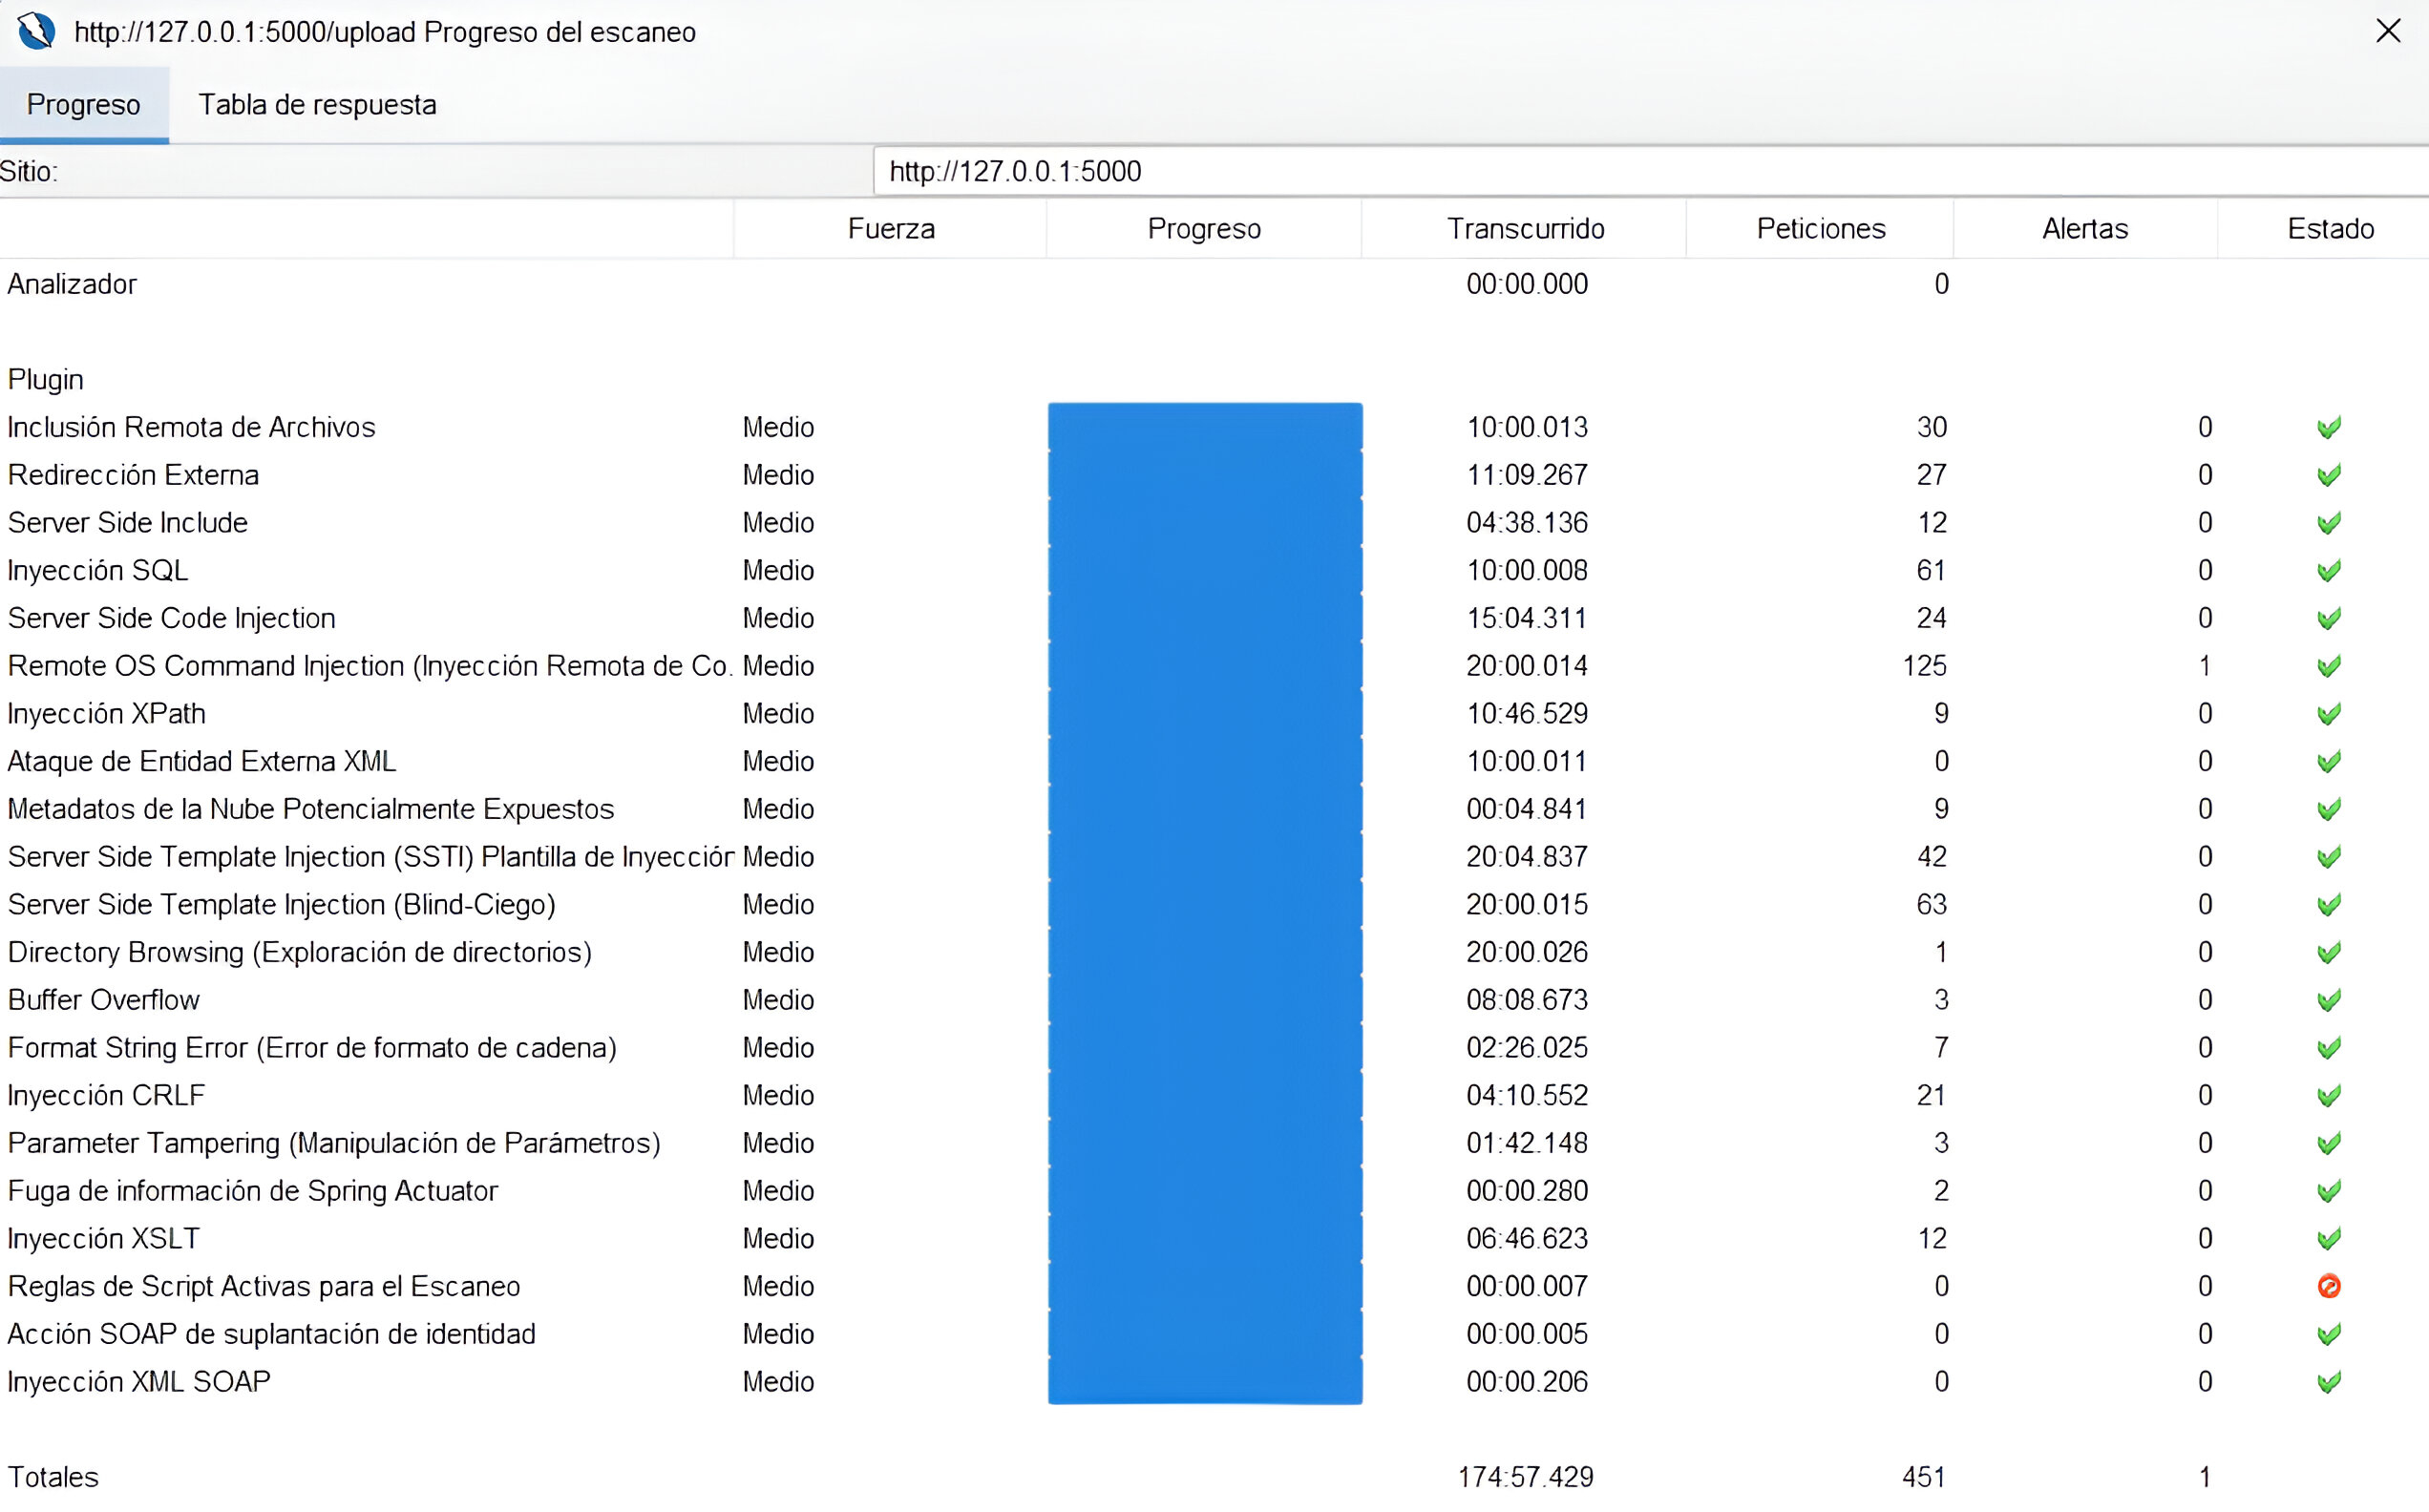
\includegraphics[width=1.0\textwidth]{figs/sec3D.jpg}
  \caption{Resultado de la prueba de seguridad sobre el endpoint del modelo generativo 3D del servidor}
  \label{fig:sec3D}
\end{figure}
En este caso, ZAP ejecutó un ataque utilizando el payload \verb|captured.jpeg';sleep 15;'|, cuya finalidad es introducir un retraso deliberado en el sistema. La herramienta interpretó la latencia observada en la respuesta como una confirmación de éxito del ataque, sin embargo, al revisar detalladamente los resultados, se observó que el servidor devolvió correctamente el modelo 3D en formato \verb|.glb|, sin ninguna anomalía funcional o sintáctica como ilustra la Figura \ref{fig:secVuln4} en la que se puede observar el cuerpo de la respuesta HTTP con los datos binarios del archivo \verb|.glb|.

% Imagen S5
\begin{figure}[h!tb]
  \centering
  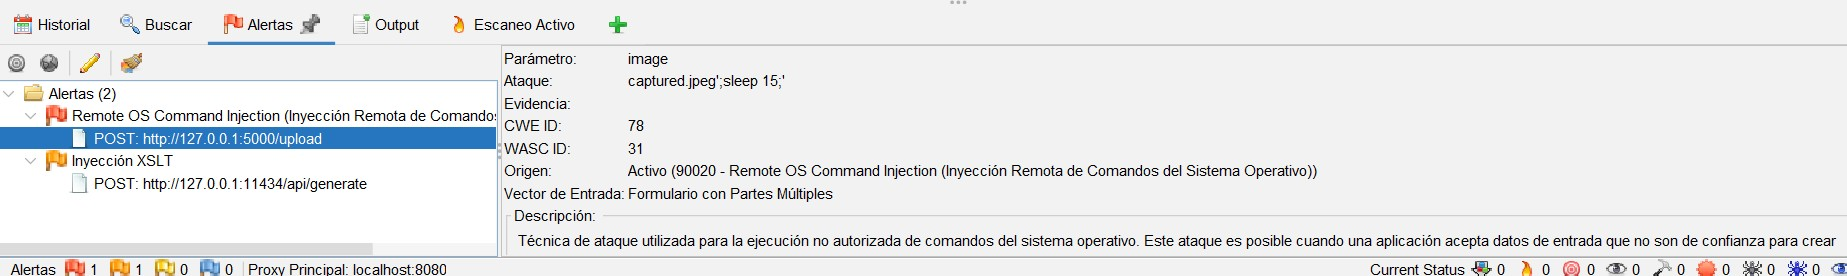
\includegraphics[width=1.0\textwidth]{figs/secVuln3.jpg}
  \caption{Vulnerabilidades obtenidas en el modelo generativo 3D}
  \label{fig:secVuln3}
\end{figure}

% Imagen S6
\begin{figure}[h!tb]
  \centering
  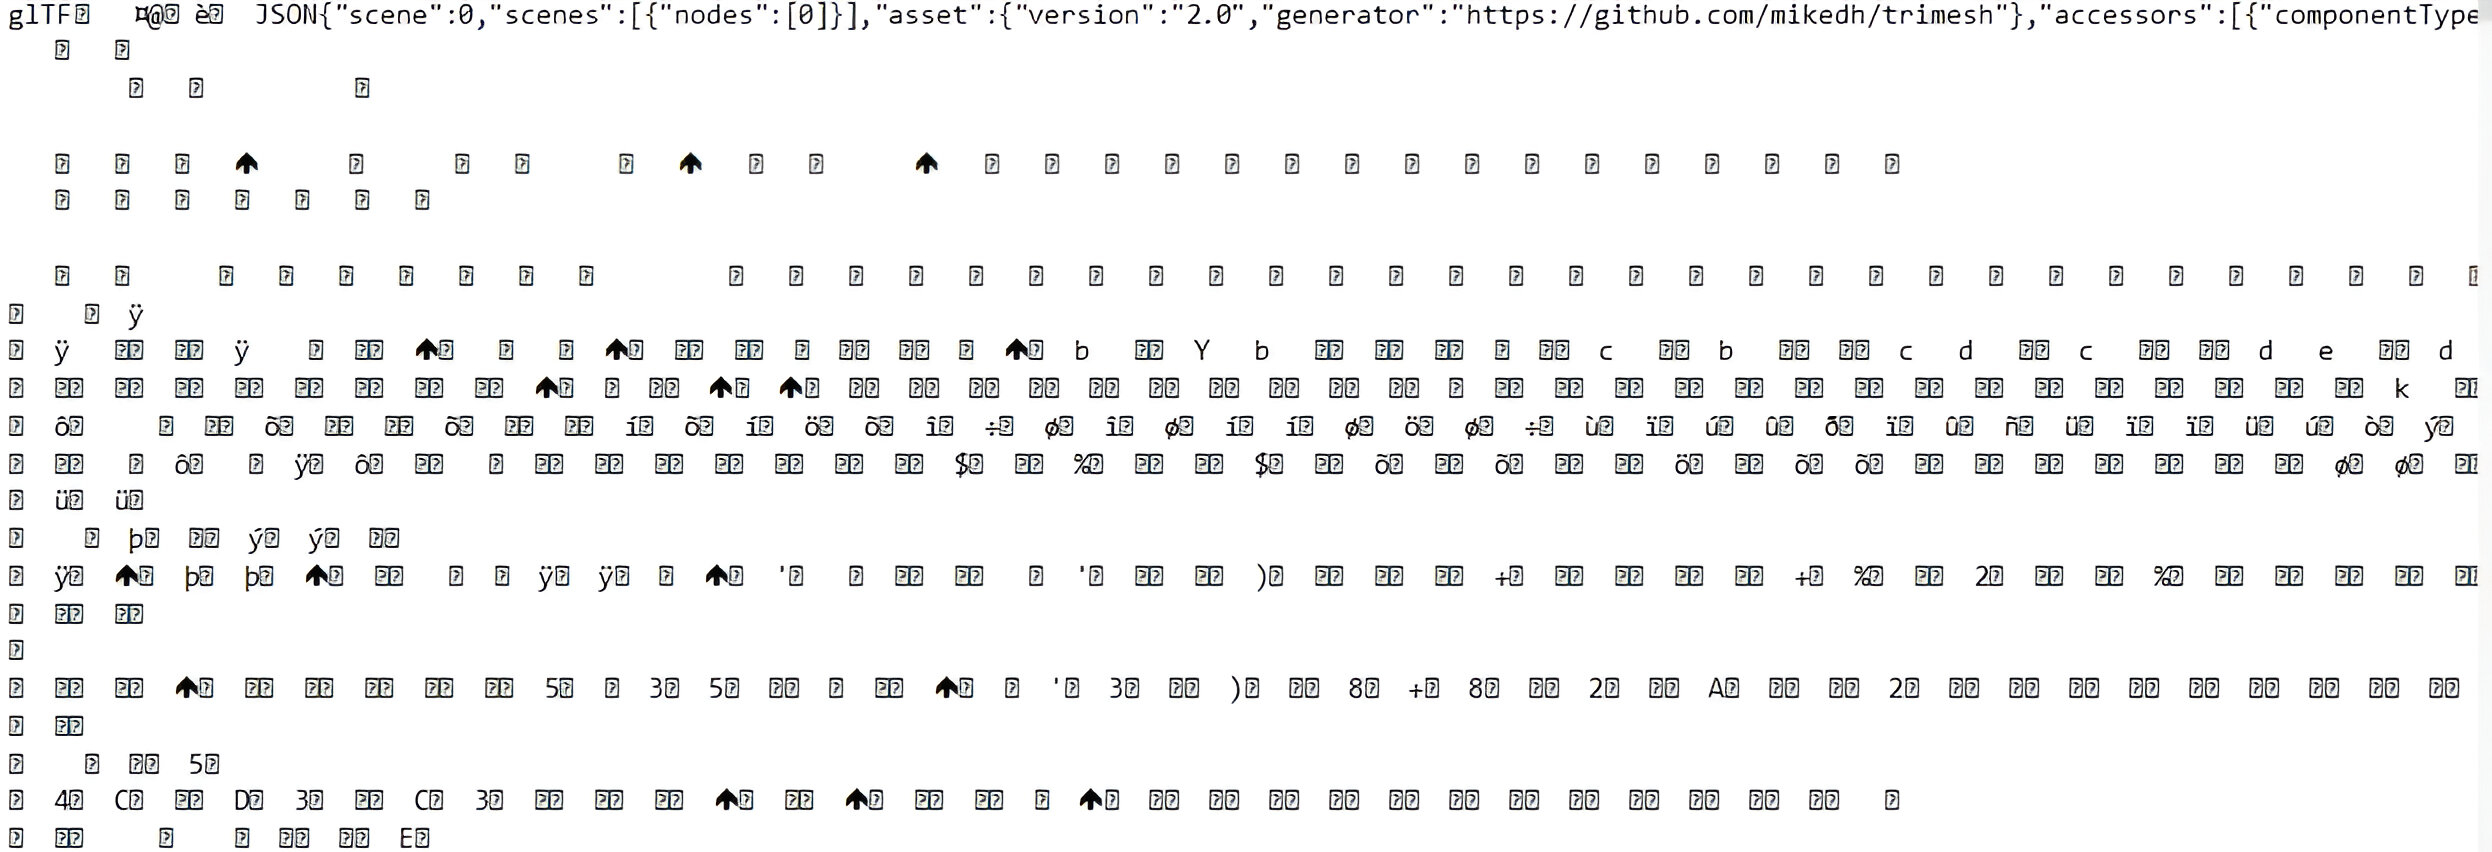
\includegraphics[width=1.0\textwidth]{figs/secVuln4.jpg}
  \caption{Detalles de la vulnerabilidad encontrada en el cuerpo de la respuesta HTTP del modelo generativo 3D}
  \label{fig:secVuln4}
\end{figure}

Adicionalmente, se intentó replicar manualmente el ataque utilizando comandos explícitos como \verb|pwd|, sin obtener ningún efecto observable, lo que sugiere que la advertencia reportada por ZAP se debe a una falsa correlación entre el tiempo de respuesta y la ejecución del comando \verb|sleep|. Dado que las pruebas de rendimiento han demostrado que el modelo generativo 3D requiere un mínimo de 40 segundos por inferencia en el mejor de los casos al estar ejecutándose en un hardware limitado, el retardo detectado por ZAP excede el umbral de los 15 segundos definidos en el payload, produciendo un falso positivo en la interpretación del test de inyección.




